%%%%%%%%%%%%%%%%%%%%%%%%%%%%%%%%%%%%%%%%%%
%Copyright (C) 2018-2020 YuZJ.
%使用CC-BY-NC-SA授权。一份完整版本的许可证已位于附录。这个版本原始作者YuZJ,
%邮箱theafamily@126.com(最后连接于2019年06月20日17:32:17)。
%%%%%%%%%%%%%%%%%%%%%%%%%%%%%%%%%%%%%%%%%%
\part{基础:计算机系统}
计算机系统(Computer System)是对是计算机正常工作的硬件和软件总称。本章将专注于基本的计算机系统,以为以后章节的操作打下基础。
\chapter{硬件}
在操作任何计算机之前,我们首先需要知道计算机的组成部分。你可以向电教员申请一台报废的计算机进行试验。\par
我们先从较为外围的设备讲起。
\section{鼠标}
\subsection{USB接口简介}
USB是“通用串行总线”的英文缩写。我们主要使用以下类型的USB接口:
\begin{enumerate}
	\item A型USB公口(Type-A)是一个标准的扁平的长方体。如果从接口外部向内部看,你会发现整个长方体一半被镂空的。它需要被插在A型USB母口(这个在计算机主机箱前面后面都能找到好几个,横截面也是标准的长方形)上。A型口在USB2.0与3.0出现一些微不足道的改变,但向下兼容。
	\begin{center}
		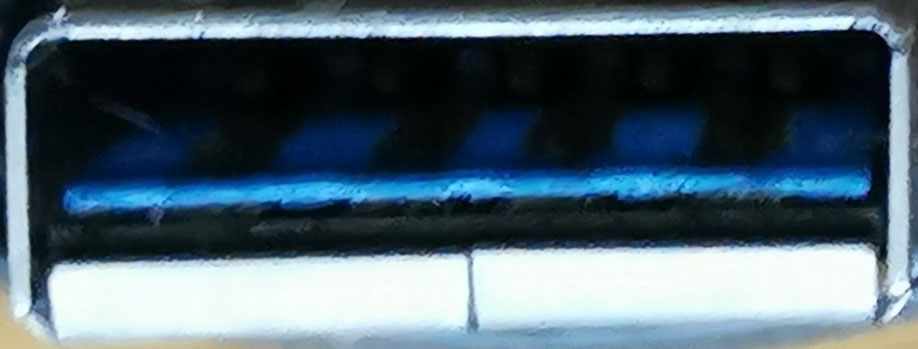
\includegraphics[width=0.7\linewidth]{pic/A-USB-1}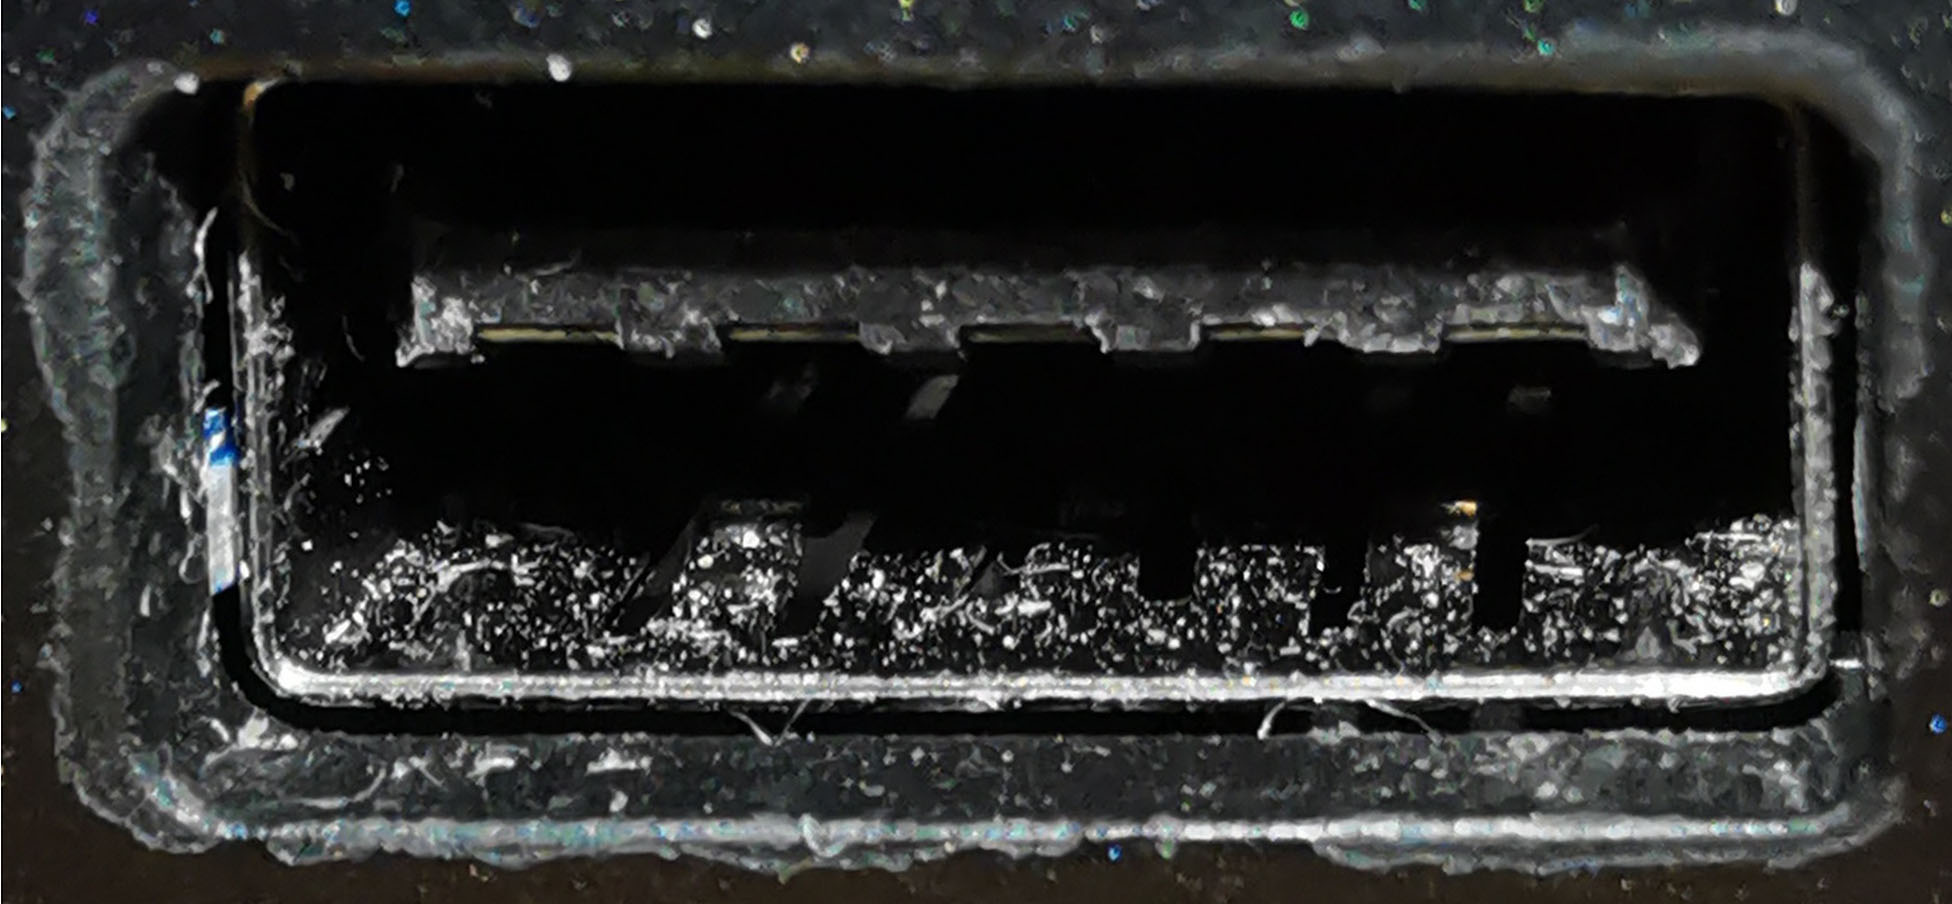
\includegraphics[width=0.7\linewidth]{pic/A-USB-2}
	\end{center}
	\item Mini-B型USB公口一般被用于移动数字设备与计算机的连接,它的截面是一个(显然被拉长的)“凸”字形结构。
	\begin{center}
		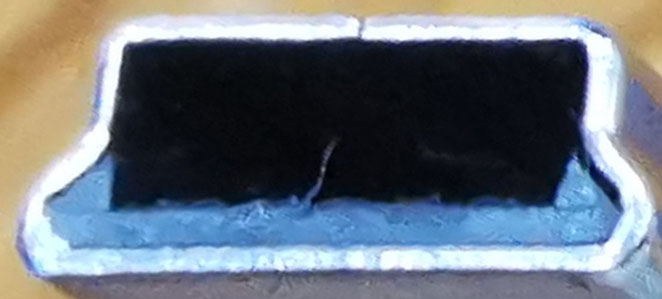
\includegraphics[width=0.7\linewidth]{pic/Mini-USB-B-1}
	\end{center}
	\item Micro-B型USB公口用途与上一种相同,但形状更接近于梯形(USB1.0-2.0)或者一个“两段体”(USB3.0+)。
	\begin{center}
		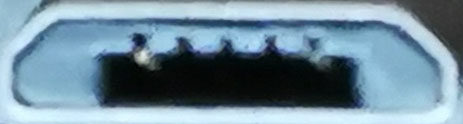
\includegraphics[width=0.7\linewidth]{pic/Micro-USB-B-1}\\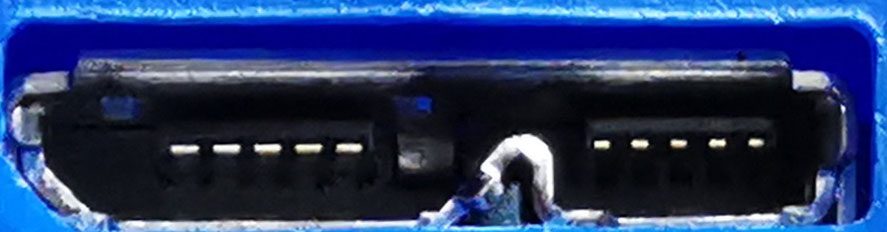
\includegraphics[width=0.7\linewidth]{pic/Micro-USB-B-2}
	\end{center}
	\item C型USB公口(Type-C)已经被用于最新的手机,它的特点是接口截面呈圆角矩形且不分正反面,且支持大电流大电压双向充电并支持转换为VGA、USB、HDMI等接口。一般仅限于USB3.0。
	\begin{center}
		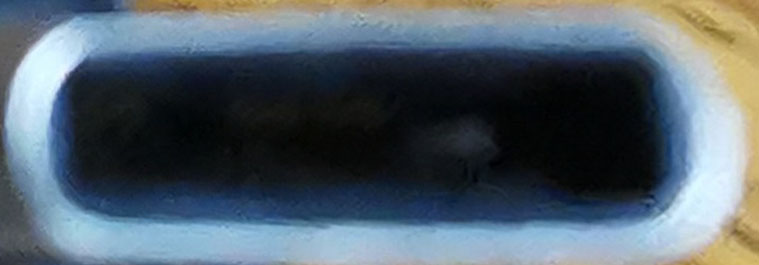
\includegraphics[width=0.7\linewidth]{pic/C-USB-1}
	\end{center}
	\item B型(Type-B)(一个长、高基本相等的图形——无论USB1.0还是3.0)主要用于打印机。
	\item Mini-A与Micro-A型USB公口不常见,但Mini与Micro各自的母口不分AB型均可插。B型USB母口不常见
\end{enumerate}
USB传输速率标准可分为1.0,2.0,3.0,3.1(目前最快标准)等。部分3.0以上的USB接口与3.0以下的接口不一样。
\subsection{鼠标的硬件结构}
顾名思义,鼠标就是形似老鼠的计算机设备。无线鼠标通常配备一个对应的USB接收器或使用蓝牙技术,有线鼠标一般使用电线连接USB或PS/2接口。一般较旧的台式机上还能看到PS/2接口。请注意PS/2插入以后需要重新启动才能生效,而USB接口一经插入即可使用。\par
你应该已经发现一般的鼠标有两个按钮(一般它们被称为“左键”和“右键”)和一个扁平的滚轮。大多数无线鼠标都需要电池,你应该先从说明书上了解这个鼠标使用何种(几号)电池以及如何安装它们。
\begin{center}
	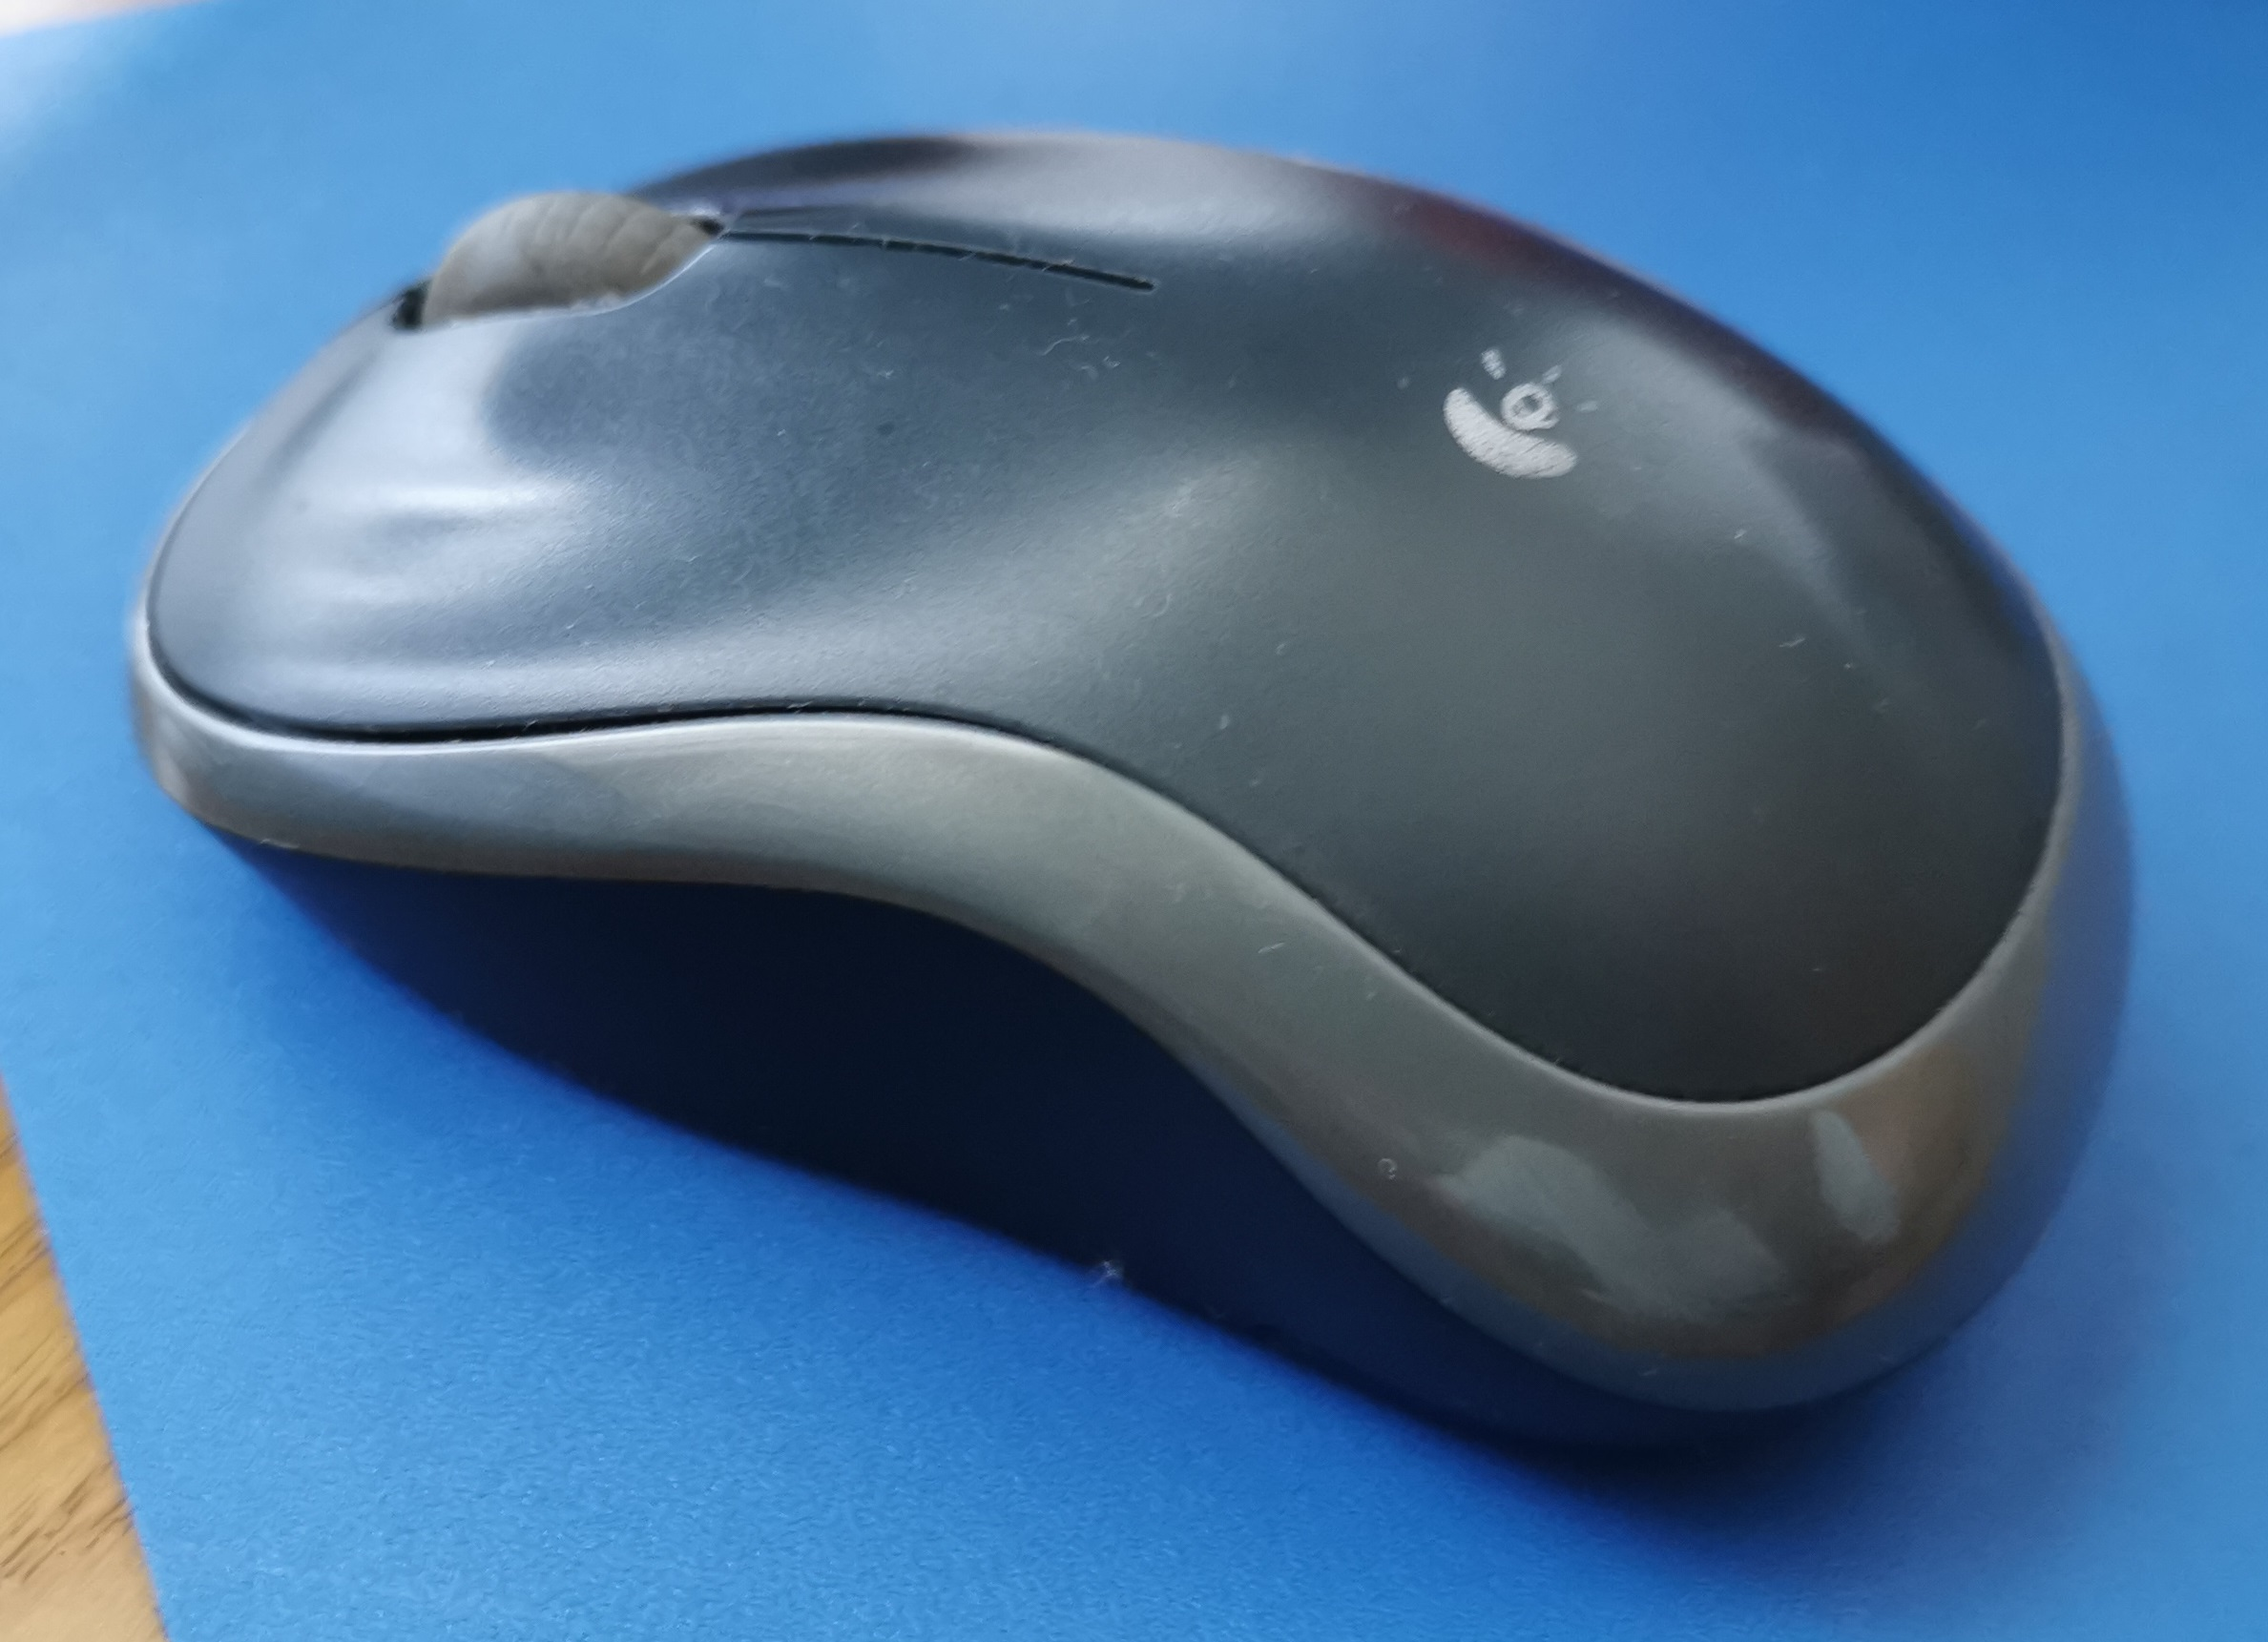
\includegraphics[width=0.7\linewidth]{pic/Mouse}
\end{center}\par
\subsection{鼠标的功能}
大多数操作系统即使没有鼠标也能完成正常运行。对于不带图形界面的GNU/Linux操作系统,鼠标是多余的。但是对于Windows操作系统或者其它带有图形界面的操作系统,鼠标的出现大大方便了用户的使用。当你的操作系统检测到鼠标以后,一个随你鼠标移动的小箭头会被显示在屏幕上,我们将其称为“光标(Cursor)”。\par
鼠标具有指向功能。安装完操作系统后将光标悬浮在应用程序上特定的部位,光标周围(也有可能是应用程序任务栏)会出现一个矩形方框,给你提供某些帮助。下图就是鼠标的指向功能的例子:你会发现已经变成“I”形的光标周围存在一个大方框,解释了“\verb|\par| ”命令的用法。
\begin{center}
	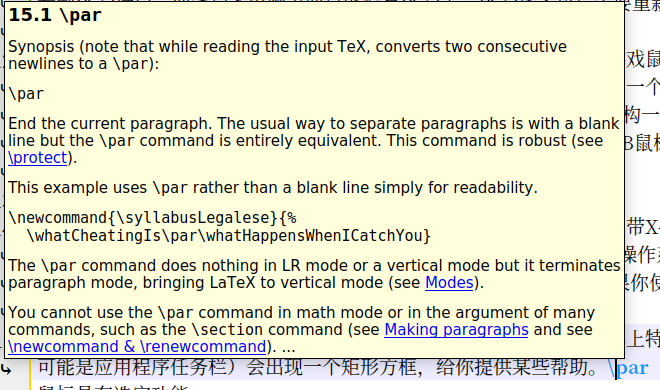
\includegraphics{pic/Crusor}
\end{center}\par
鼠标具有选定功能。双击桌面上的图标以打开“文件资源管理器”。如果你在默认的文件资源管理器单击(就是用左键点击一下)一个图标(比如说C盘),光标颜色将改变并进入“选定”状态。此时如果你的文件资源管理器具有“预览”窗格,它将会显示关于这个图标所代表的文件或者文件夹的详细信息。如果你双击(就是用左键快速单击两下)它,被选定的文件将被打开。资源管理器为你显示了驱动器内的内容。同样地,你也可以这样打开文件夹和文件。现在对一个驱动器、文件或文件夹右击,一个菜单将会被弹出。这种菜单被称为“文件资源管理器右键菜单”。对于菜单中内容请参见\pageref{Sec:FE}页的\ref{Sec:FE}。
\subsection{使用鼠标}
如果你希望使用左手,请使用左手专用鼠标。下文仅以右手鼠标为例。\par
请将鼠标放置在粗糙的表面上(如鼠标垫),右手握鼠标。在安装完操作系统以后,将鼠标插入计算机(并重启,针对PS/2鼠标)。请检查你鼠标的说明书了解是否需要安装特定的驱动程序(虽然大多数鼠标都是即插即用的),如果需要请安装(使用键盘)。正确配置以后,你的桌面上应该出现一个光标。移动鼠标,如果光标随着鼠标移动并能响应单击等操作,鼠标的基本配置就完成了。\par
现在配置鼠标。单击“开始”菜单-设置(齿轮)-设备-鼠标。你在那里可以修改主按钮(“左键”)、一次滚动行数等。在“设置”的轻松使用-光标和指针修改光标大小和颜色与键入时光标大小,在控制面板(“开始”菜单-Windows系统-控制面板)-硬件和声音-设备和打印机-鼠标来修改鼠标双击速度、指针类型和选项、指针轨迹等。
\section{键盘}
\subsection{键盘的硬件结构}
一块用于键入字符的板是键盘。请注意,一台计算机可以没有鼠标,但不能没有键盘!\par
按照键位分类,最常见的键盘是QWERTY键盘。这种键盘中,第一排为包含“ESC”,“F1”到“F12”的功能键区,第二排是“~”、“1”到“9”、“0”、“-”“=”与“退格”(一般被标注为“Backspace”或“$\leftarrow$”),第三排是制表符(一般被标注为“Tab”)和“Q”“W”“E”“R”“T”“Y”“U”“I”“O”“P”“[”“]”“\textbackslash”,第四排是“大写锁定”(一般被标注为“CapsLock”或“Caps”)和“A”“S”“D”“F”“G”“H”“J”“K”“L”“;”“'”与“回车”(一般被标注为“Enter”或“$\hookleftarrow$”),第五排是“上档”(一般被标注为“Shift”或“$\uparrow$”)与“Z”“X”“C”“V”“B”“N”“M”“,”“.”“/”与另一个Shift键,第六排是“控制”(一般被标注为“Ctrl”)、“功能”(一般被标注为“Fn”,有可能在控制键左边或不存在。)、“Windows”(一般被标注为键盘生产时最新版本Windows操作系统的徽标)、“交替换挡”(一般被标注为“Alt”)、“空格”(长方块,有时标有“Space”或者“\verb*| |”)、另一个Alt、另一个Windows、菜单键与另一个Ctrl。在主键盘右侧最上一排(系统键区)是“截屏”(一般被标注为“PrtSc”或“PrtScr”)、“滚动锁定”(一般被标注为“Scroll Lock”)、“暂停”(一般被标注为“Pause Break”),第二排(编辑键区)为“插入”(一般被标注为“Insert”)、“主界面”(一般被标注为“Home”)、向上翻页(一般被标注为“PageUp”),第三排(编辑键区)为“删除”(一般被标注为“Delete”或“Del”,以下简称“Delete键”)\footnote{注意,对于“删除”键的定义,不同的程序是不同的。比如说GNU Emacs就把退格键定义为删除键。}、“结束”(一般被标注为“End”)、“向下翻页”(一般被标注为“PageDown”)。下一行有四个方向键,最右边是数字键盘(笔记本一般是没有的)。\par
键盘按照接口也分USB与PS/2(同样需要重启)。笔记本上一些键是蓝色的,此时就应先按住Fn键再按需要的键。请注意对于USB接口,一部分操作系统(如Windows XP)的安装会受到阻碍。
\begin{center}
	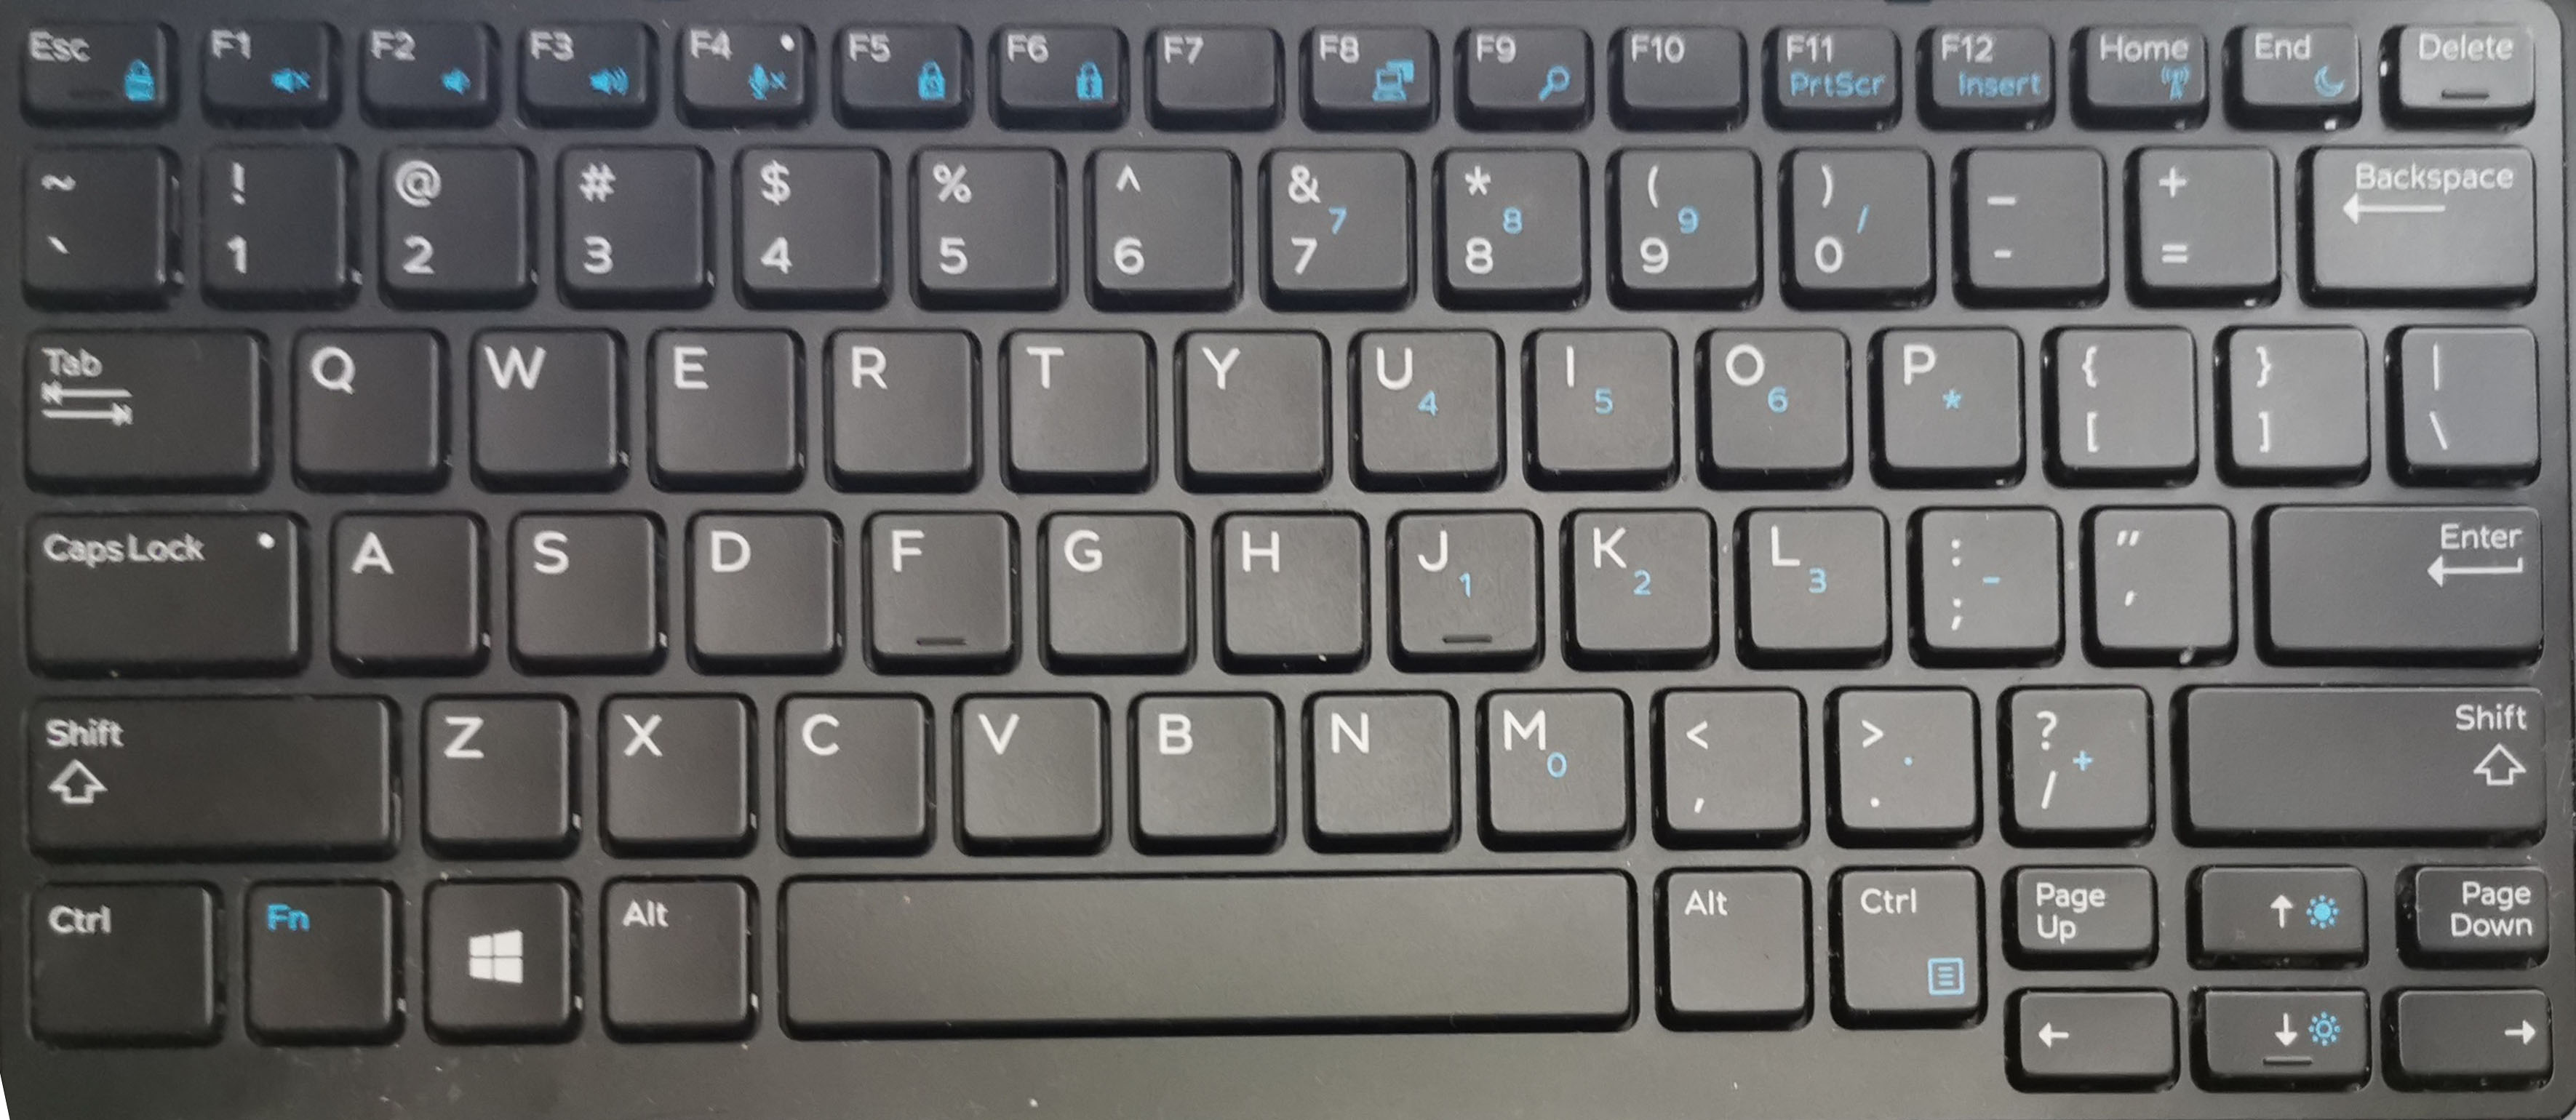
\includegraphics[width=0.7\linewidth]{pic/KB1}\\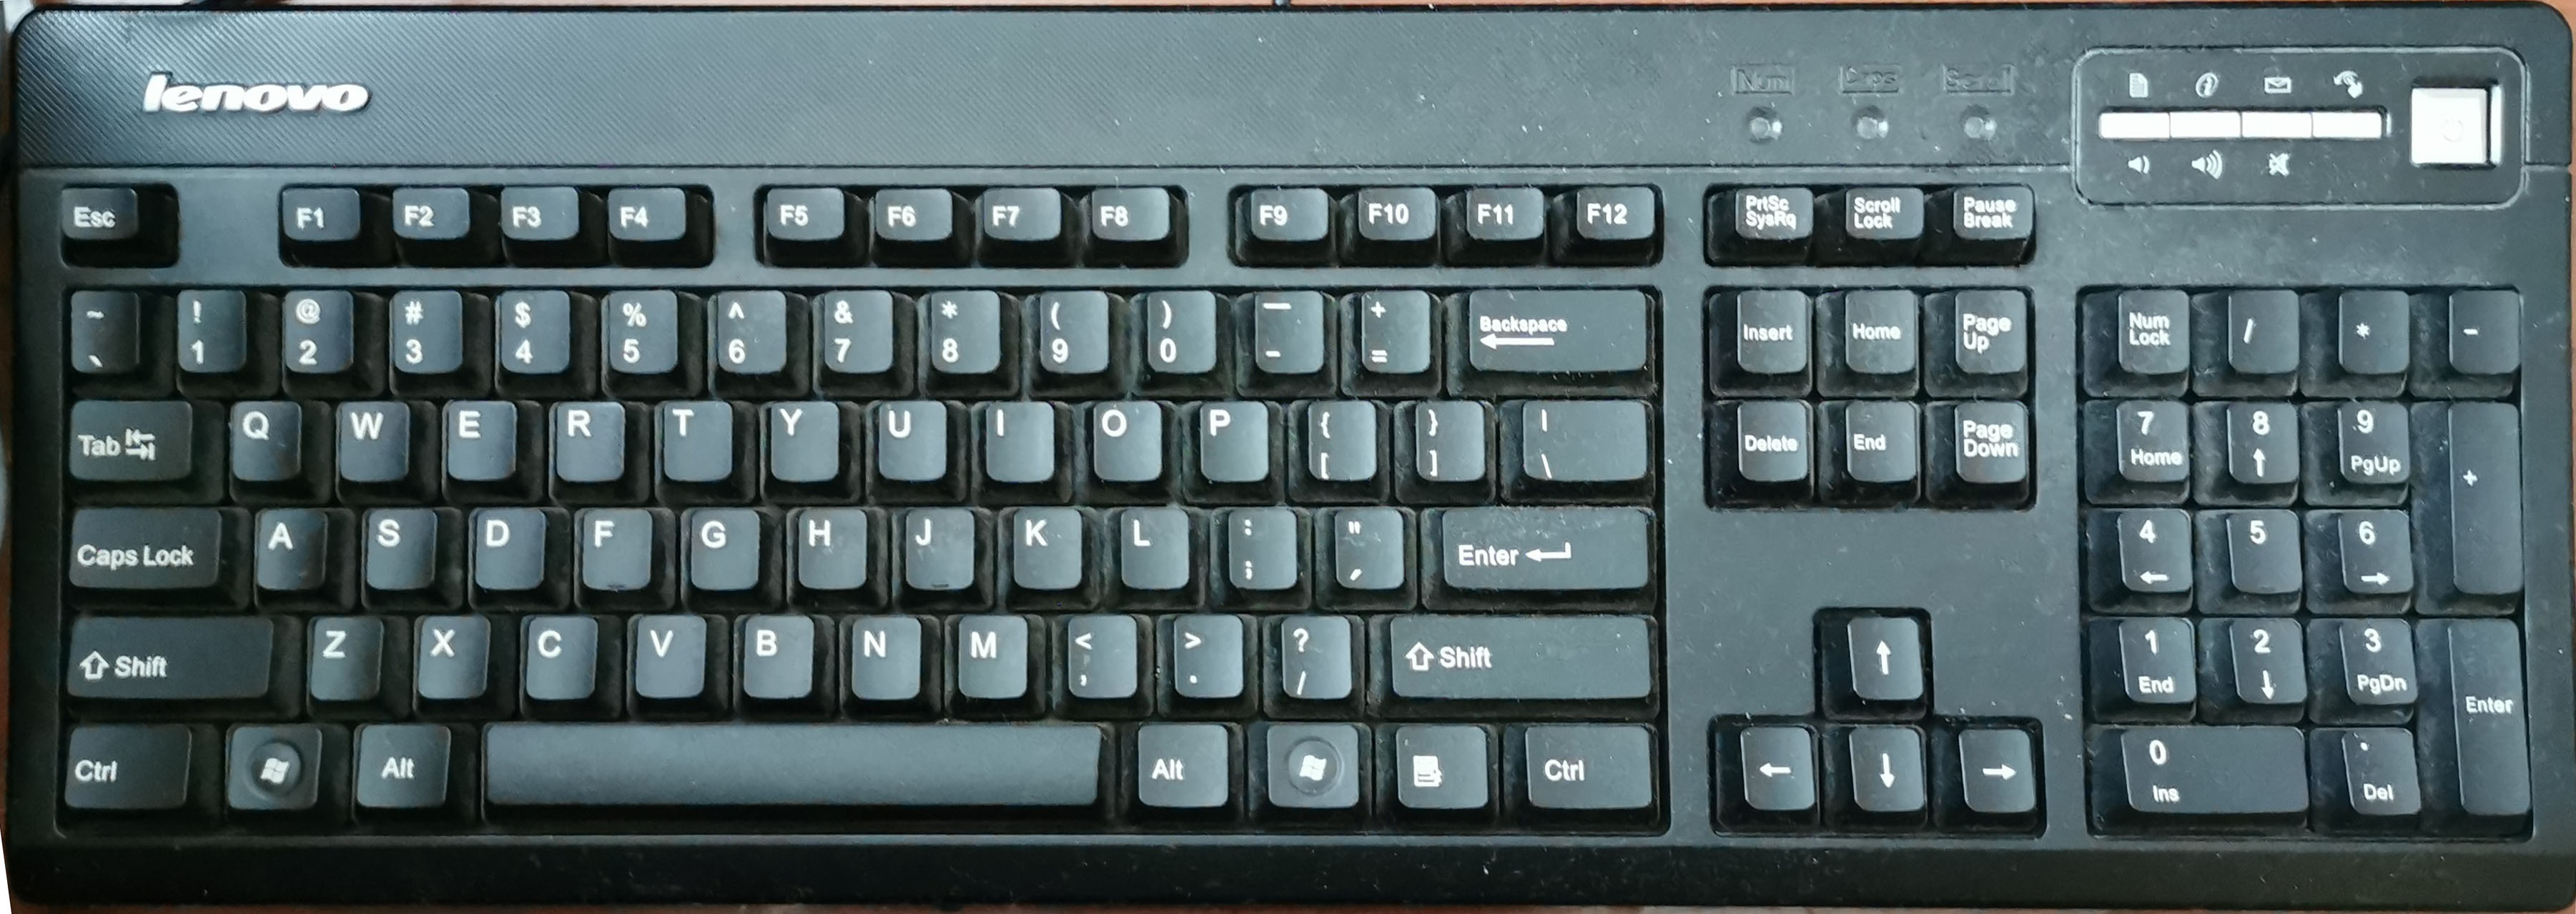
\includegraphics[width=0.7\linewidth]{pic/KB2}
\end{center}\par
\subsection{焦点、活动窗口与快捷键}
活动窗口就是你当前正在操作(或者你最后一个操作)的窗口。比如说现在你正在阅读本书的电子版,那么你的PDF阅读器所在的窗口就是活动窗口。之后你打开了文件资源管理器,文件资源管理器窗口就是活动窗口。\par
焦点是一个活动窗口上的活动控件(具体参见\pageref{sec:Frm}页的\ref{sec:Frm}章节)。比如说这样一个有一个文本框与两个按钮的窗口:\par
\begin{center}
	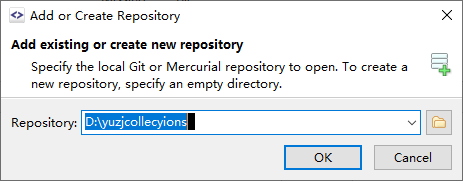
\includegraphics[width=0.7\linewidth]{pic/forcus1}
\end{center} \par
按下“Tab”键:\par
\begin{center}
	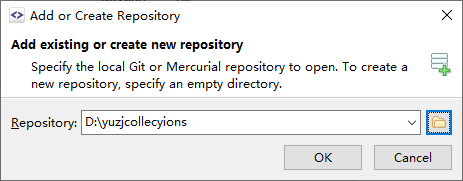
\includegraphics[width=0.7\linewidth]{pic/forcus2}
\end{center} \par
\begin{center}
	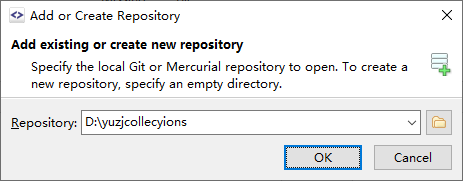
\includegraphics[width=0.7\linewidth]{pic/forcus3}
\end{center} \par
焦点就被切换了。Tab键是切换焦点的最佳键。注意,焦点和活动窗口具有唯一性。请注意第一个图像上的“OK”按钮具有“默认”属性此时在这个窗口上按下回车键就相当于按下这个键\par
在Widows操作系统上你可以使用一些特别的快捷键。在下面的表格里面,“C-”表示你需要按住控制键(“Ctrl”)时按短线后的键,“M-”则是按住Alt键\footnote{为了与GNU Emacs的快捷键称法一致,我们使用“M”。},“Win”表示Windows键,“Del”表示Delete键,“S”为Shift键,“Space”为空格键,“U”“D”“L”“R”为上、下、左、右四个方向键。
\begin{verbatim}
F1        显示帮助
F2        当“文件资源管理器”中一个文件被选中时,可以重命名
F5        刷新
F10       系统启动时显示BIOS(一般情况)
F12       系统启动时显示临时启动菜单
C-c       复制
C-v       粘贴
C-x       剪切
C-z       撤销
C-S       切换输入法(GNU/Linux下Fcitx平台默认“C-Space”)
C-M-Del   进入“安全选项”(其中可以叫出任务管理器)
Windows XP为叫出任务管理器,部分GNU/Linux为直接重启
M-F4      关闭窗口
M-Space   窗口控制菜单
M-Tab     切换活动窗口
Win       打开“开始”菜单
Win-b     将焦点移到任务栏托盘区
Win-d     显示桌面
Win-l     锁定计算机
Win-m     最小化所有窗口
Win-r     打开“运行”
Win-U     最大化活动窗口(让这个窗口铺满整个屏幕)
Win-D     最小化活动窗口(让这个窗口消失到任务栏)
Win-Home  最小化除活动窗口外所有窗口
\end{verbatim}
\section{机箱}
机箱是一个方形铁盒子,上面有一个电源按钮必须的接口。
\subsection{电源按钮}
电源按钮就是你需要在开机时按下的按钮。这个按钮有两个功能:1.开机。2.当你的计算机死机或者由于其它原因你需要强行关闭此计算机时,你可以长按这个按钮。这将导致计算机被强行关闭({\color{red}警告!正常情况下不要尝试使用这种方法关闭计算机——这有可能导致严重的数据丢失!})。
\begin{center}
	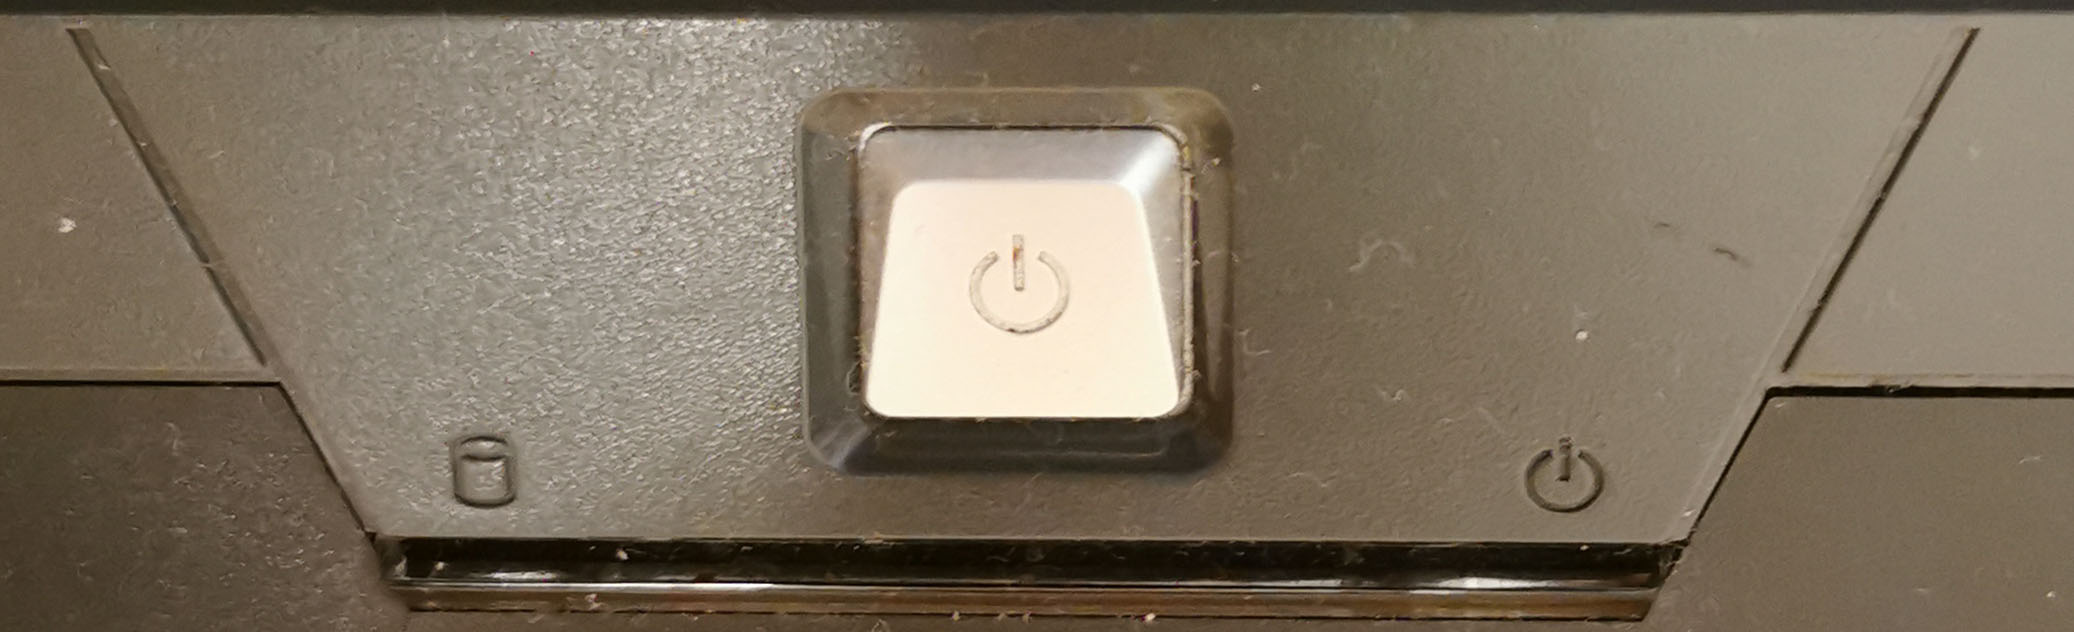
\includegraphics[width=0.7\linewidth]{pic/StB}
\end{center}\par
“复位”按钮是一个小型的按钮,上面标有“Reset”或者其他东西——这个按钮的作用是在主板上通电来使主板强制重启。{\color{red}警告!不要尝试使用这种方法关闭计算机——这有可能导致严重的数据丢失!}有些主机没有这个按钮。
\subsection{接口}
我们先从前面板讲起。\par
3.5mm TRS接口。前面板上面的两个直径小于5mm的圆形接口就是了。这是3.5mm TRS(“三段式”)接口。这两个接口的作用是连接耳机和麦克风。一般绿色的是耳机,红色的是麦克风。与它适配的耳机或麦克风接口表面上有有2个“环”。还有一些新机器装备的是TRRS(“四段式”)接口。TRRS的接口比TRS多一个“环”,能同时传播耳机与麦克风信号。这种设备对应的声卡需要你选择插入的是耳机、麦克风还是耳麦。
\begin{center}
	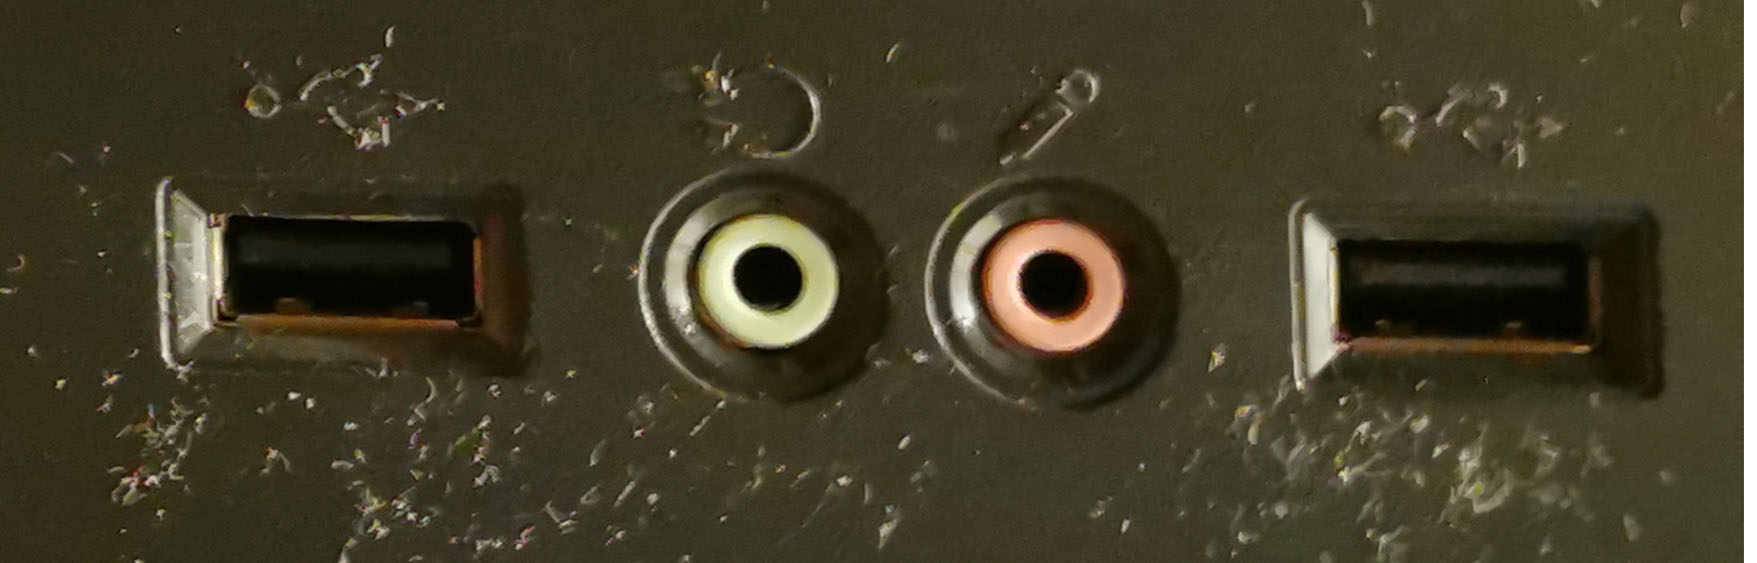
\includegraphics[width=0.7\linewidth]{pic/Box1}
\end{center}\par
现在开始讲后面板,顺序从上到下。\par
电源接口。一个被截取两个角的矩形,内有三根金属插座。这是电源盒与电源线的连接口。
\begin{center}
	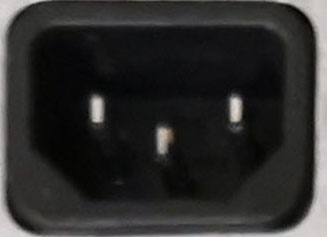
\includegraphics[width=0.7\linewidth]{pic/Power}
\end{center}\par
一对PS/2接口。用于鼠标与键盘。
\begin{center}
	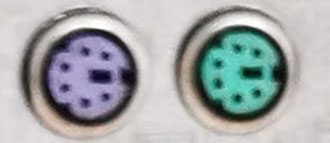
\includegraphics[width=0.7\linewidth]{pic/PS2}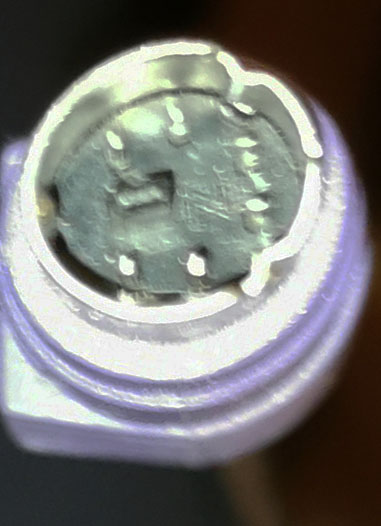
\includegraphics[width=0.7\linewidth]{pic/PS2L}
\end{center}\par
VGA接口。一个较扁的圆角梯形接口,内部有许多可插“针”的小孔。这是用于显示器的接口,适用于较低分辨率(1920$\times$1200以下)显示器。VGA接口旁边还有两个固定螺栓注意,这个接口传输的是模拟信号。\begin{center}
	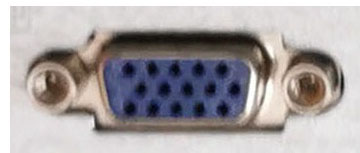
\includegraphics[width=0.7\linewidth]{pic/VGA}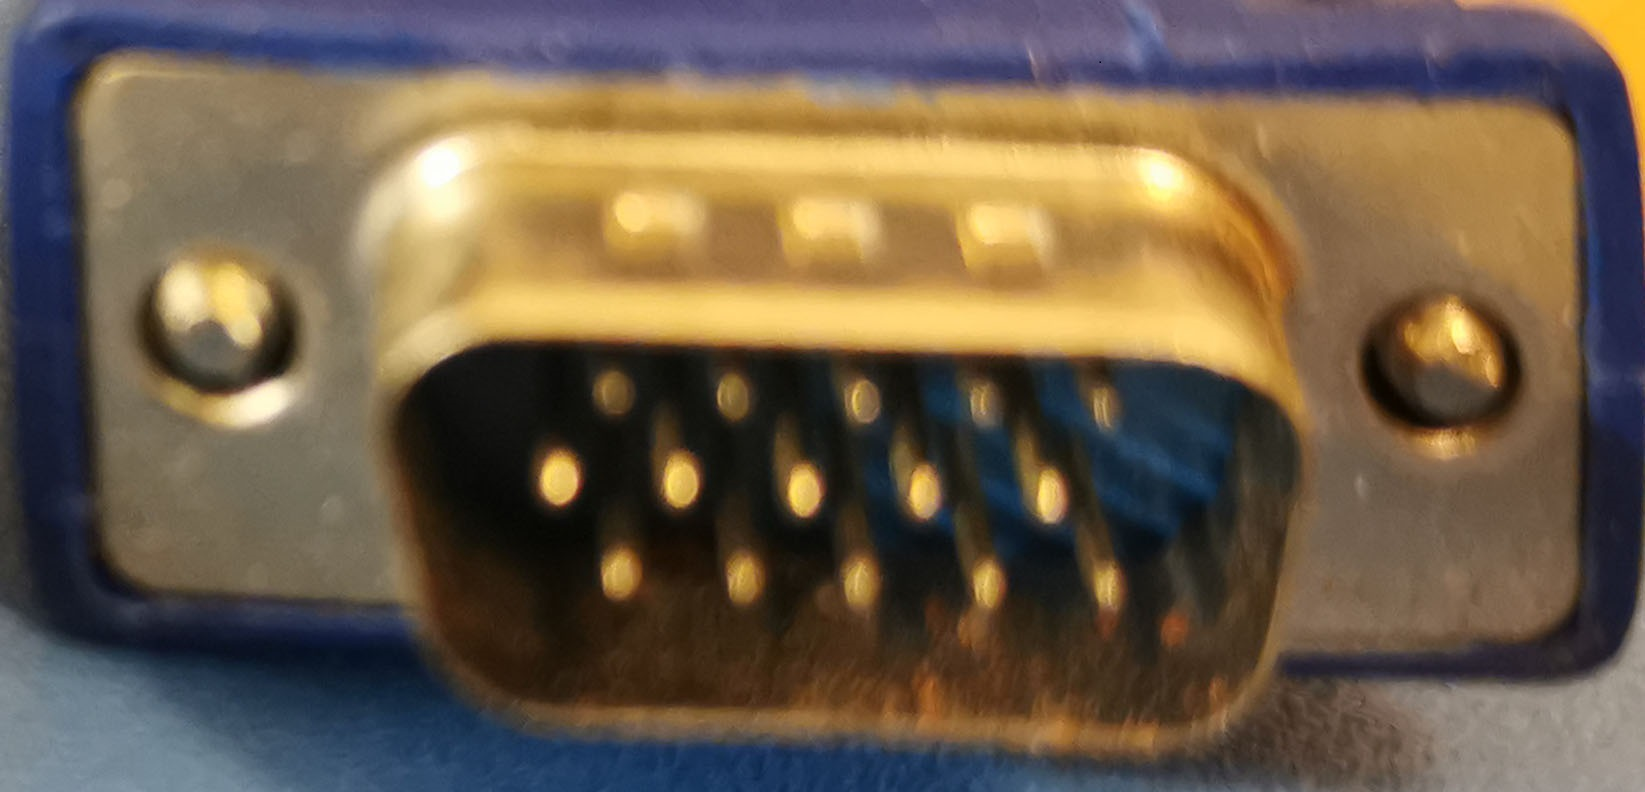
\includegraphics[width=0.7\linewidth]{pic/VGAL}
\end{center}\par
HDMI接口。一个较扁的梯形与矩形的结合物。一种能传播音频信号的高清显示接口。
\begin{center}
	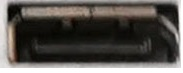
\includegraphics{pic/HDMI}
\end{center}\par
DVI接口。较扁的接口,类似于截取两个角矩形,内部有许多针。一种高清显示接口。\par
6个A型接口USB接口。有些笔记本有C型USB接口。
\begin{center}
	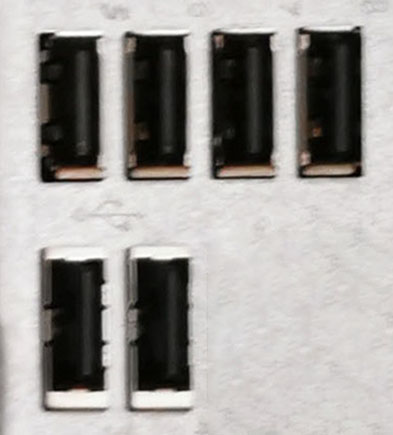
\includegraphics[width=0.7\linewidth]{pic/USB}
\end{center}\par
RJ-45接口。一个较方的,内含多个金属引脚的接口。这是用于网线(“双绞线”)的插头(“水晶头”)的接口。水晶头插入后可以被牢牢地固定好。
\begin{center}
	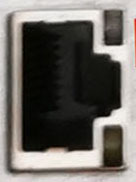
\includegraphics[width=0.7\linewidth]{pic/RJ}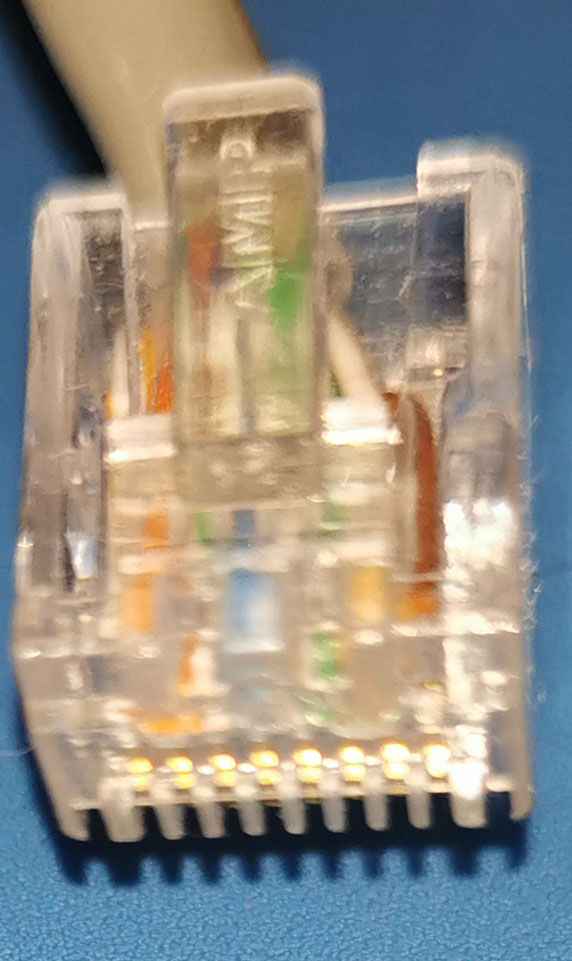
\includegraphics[width=0.7\linewidth]{pic/RJL}
\end{center}\par
2个3.5mm TRS接口。
\begin{center}
	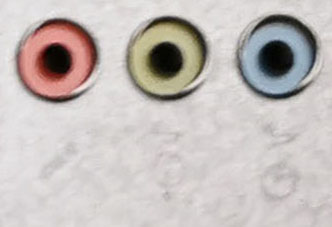
\includegraphics[width=0.7\linewidth]{pic/TRS}
\end{center}\par
几个槽(一般被封闭起来),用来连接PCI或PCI-E设备。
\section{显示器}
显示图像的地方。分辨率按宽高比分为4:3(方的)与16:9(长的)。一般目前主流是16:9。显示器有几个重要参数:分辨率(能显示图案的清晰度)与刷新频率(一秒钟显示图像数量)。具体设置方法参照显示器说明书。
\section{移动硬盘和U盘}
这是外置存储设备。一般来说,U盘的容量小于硬盘,但大容量U盘也不是不可能。以下是我曾经使用的U盘和移动硬盘,请大家格外注意USB接口。
\begin{center}
	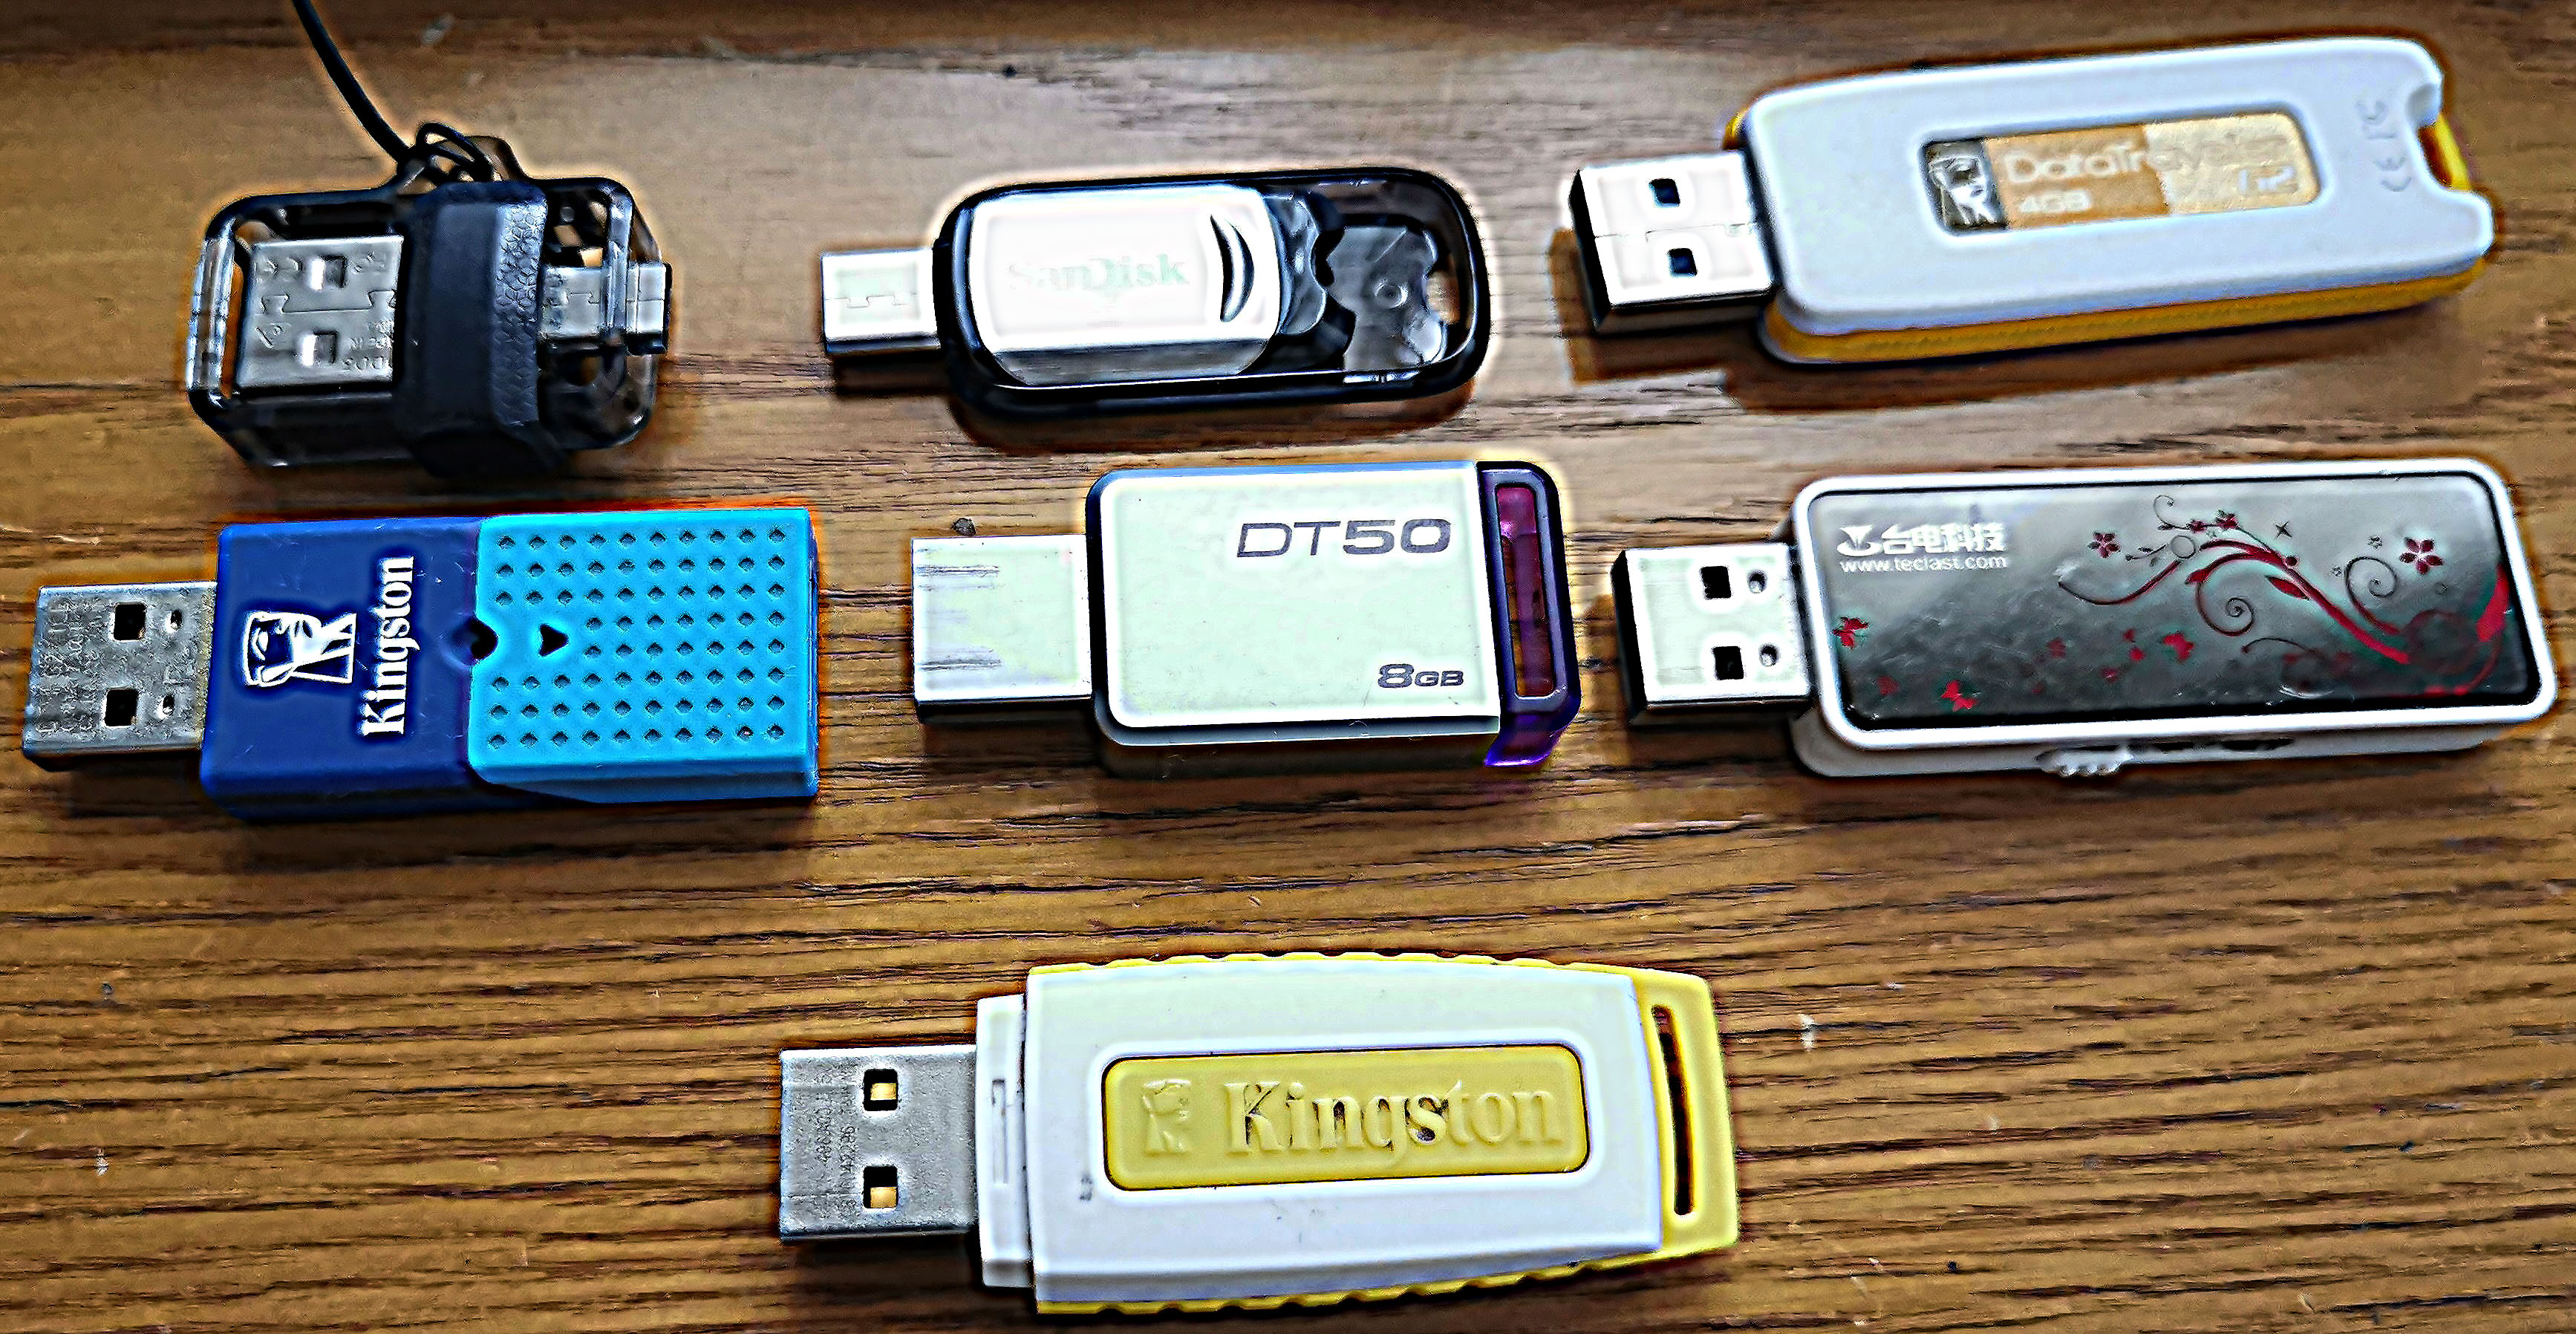
\includegraphics[width=0.7\linewidth]{pic/FlashDisk1}	\\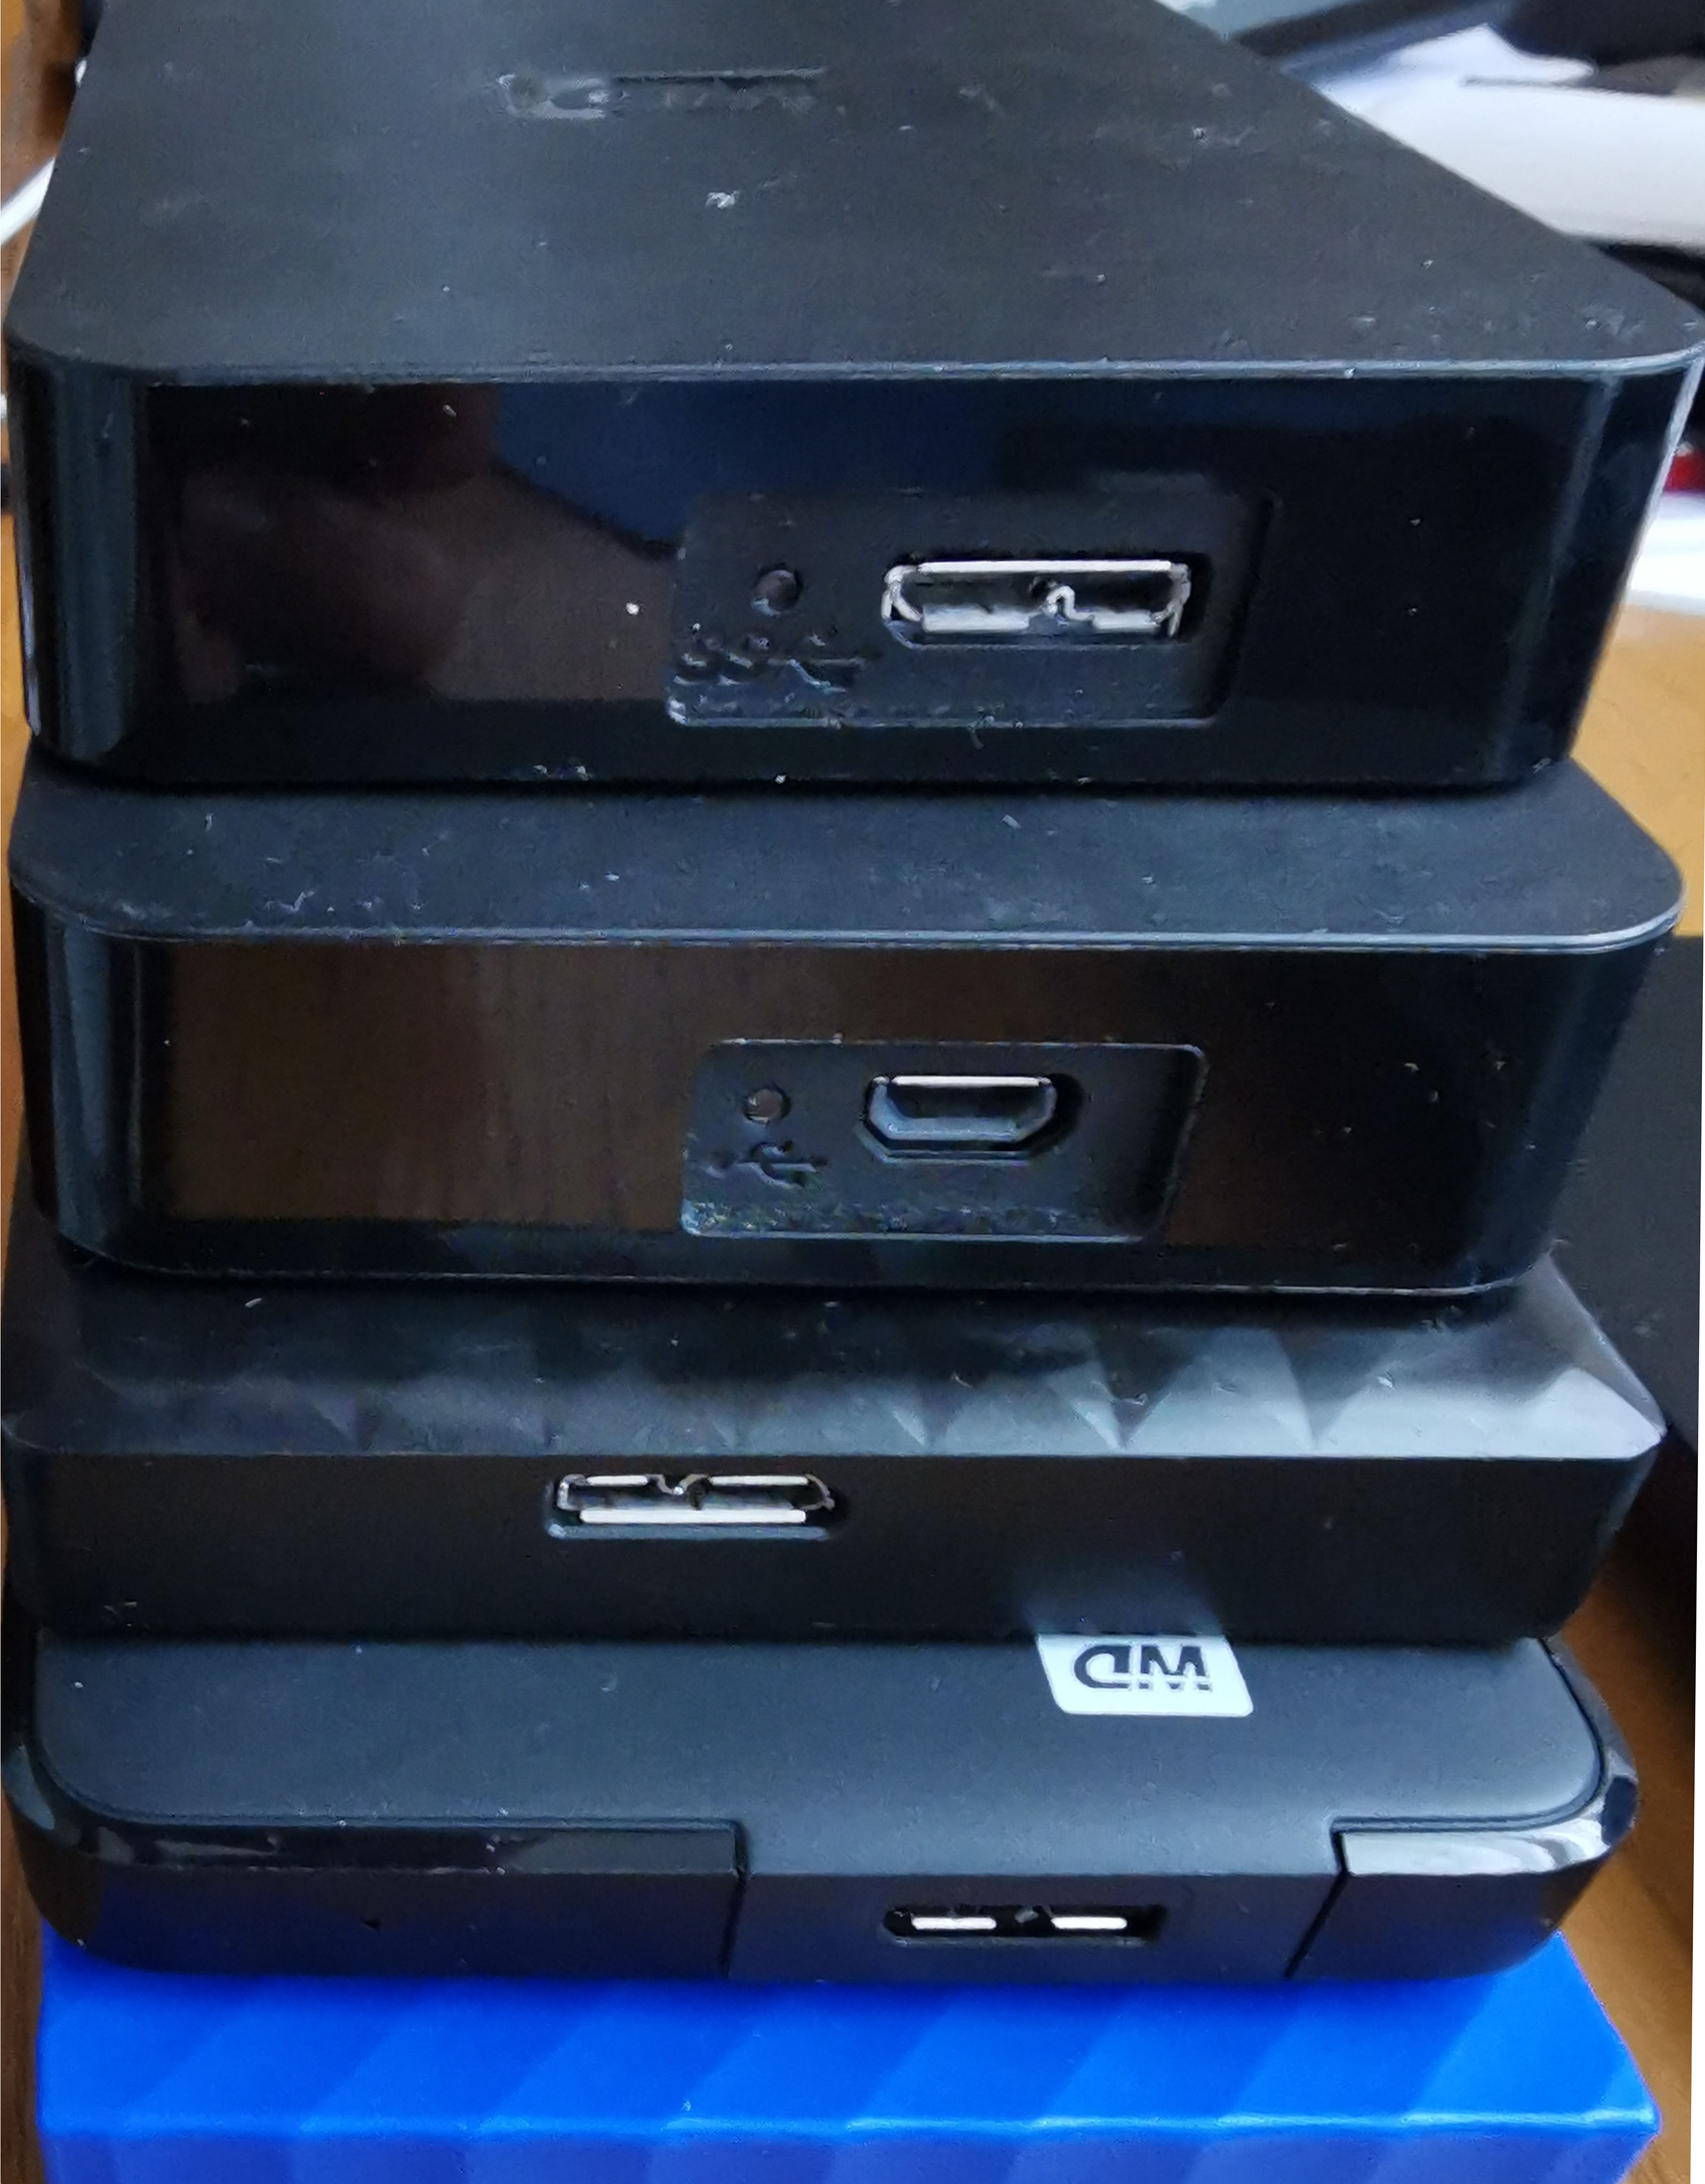
\includegraphics[width=0.7\linewidth]{pic/FlashDisk2}
\end{center} \par
现在讲一讲固态硬盘与机械硬盘。机械硬盘将信息存储在磁片上,靠磁片高速转动来读取数据。固态硬盘类似于U盘,将信息存储在芯片上。相较于机械硬盘,固态硬盘寿命较短且价格较高,但不易摔坏且速度极快,适合用于安装操作系统。机械硬盘价格便宜,适合储存大量数据(如文档)。下图是SATA接口的固态硬盘和机械硬盘。
\begin{center}
	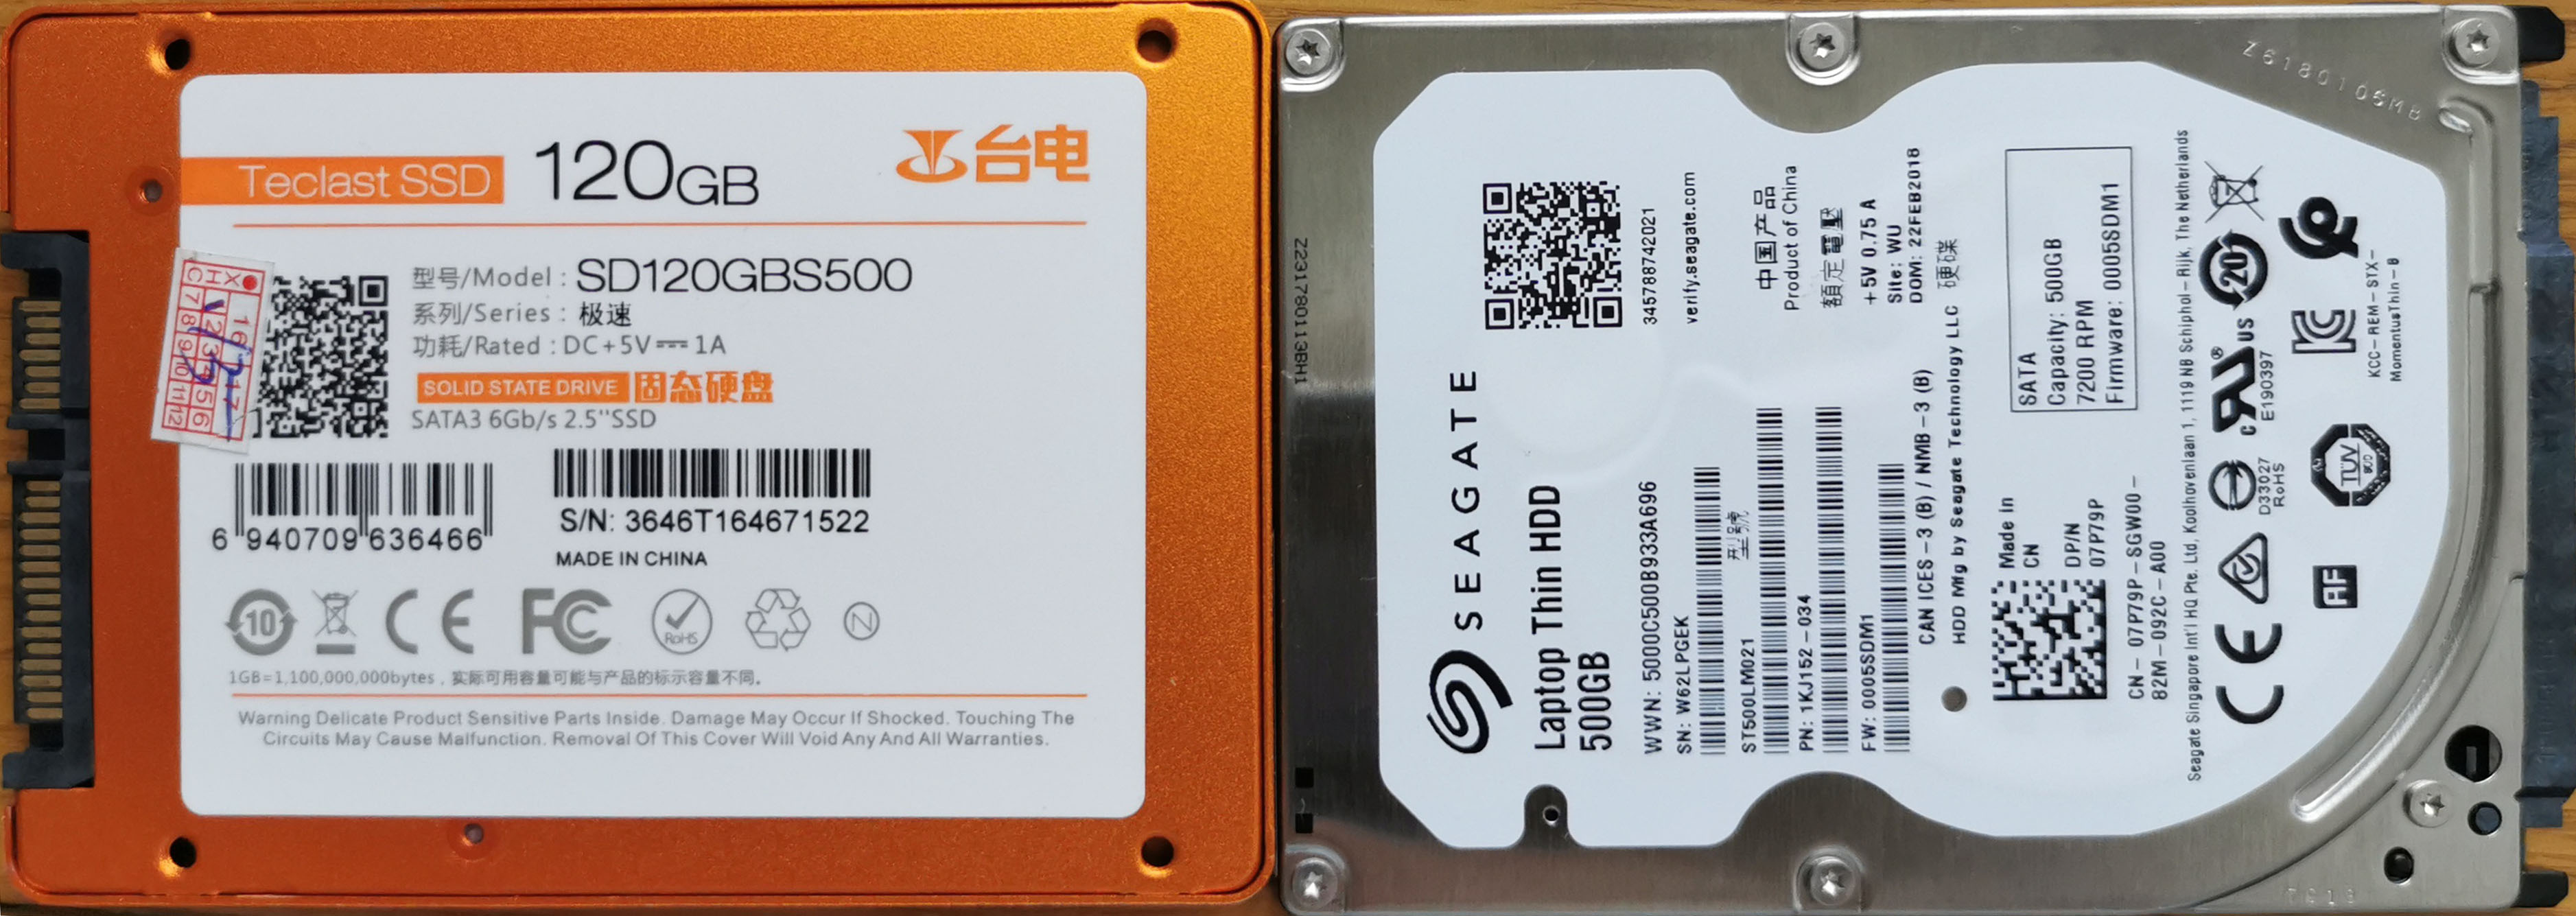
\includegraphics[width=0.7\linewidth]{pic/HD}
\end{center} 
\section{触摸板}
相当于鼠标,笔记本电脑的标配。靠手指移动代表鼠标滑动。大部分都有左右键,有些存在滚动条以模拟滚轮功能。触摸板支持滚动(双指向滚动方向运动)和缩放(双指张开/捏合)等操作。
\section{内置硬盘}
主要功能仍然是存储数据,也分固态与机械,但接口与尺寸有特定规范。\par
先说接口。主要有以下几种:
\begin{enumerate}
	\item IDE是较为老式的接口,传输速率慢,数据线线较短。它的电源接口矩形,内有4根粗针,数据接口矩形,内有2排每排20共40针,矩形的长边上有一个缺口。下图的IDE接口有断针。
	\begin{center}
		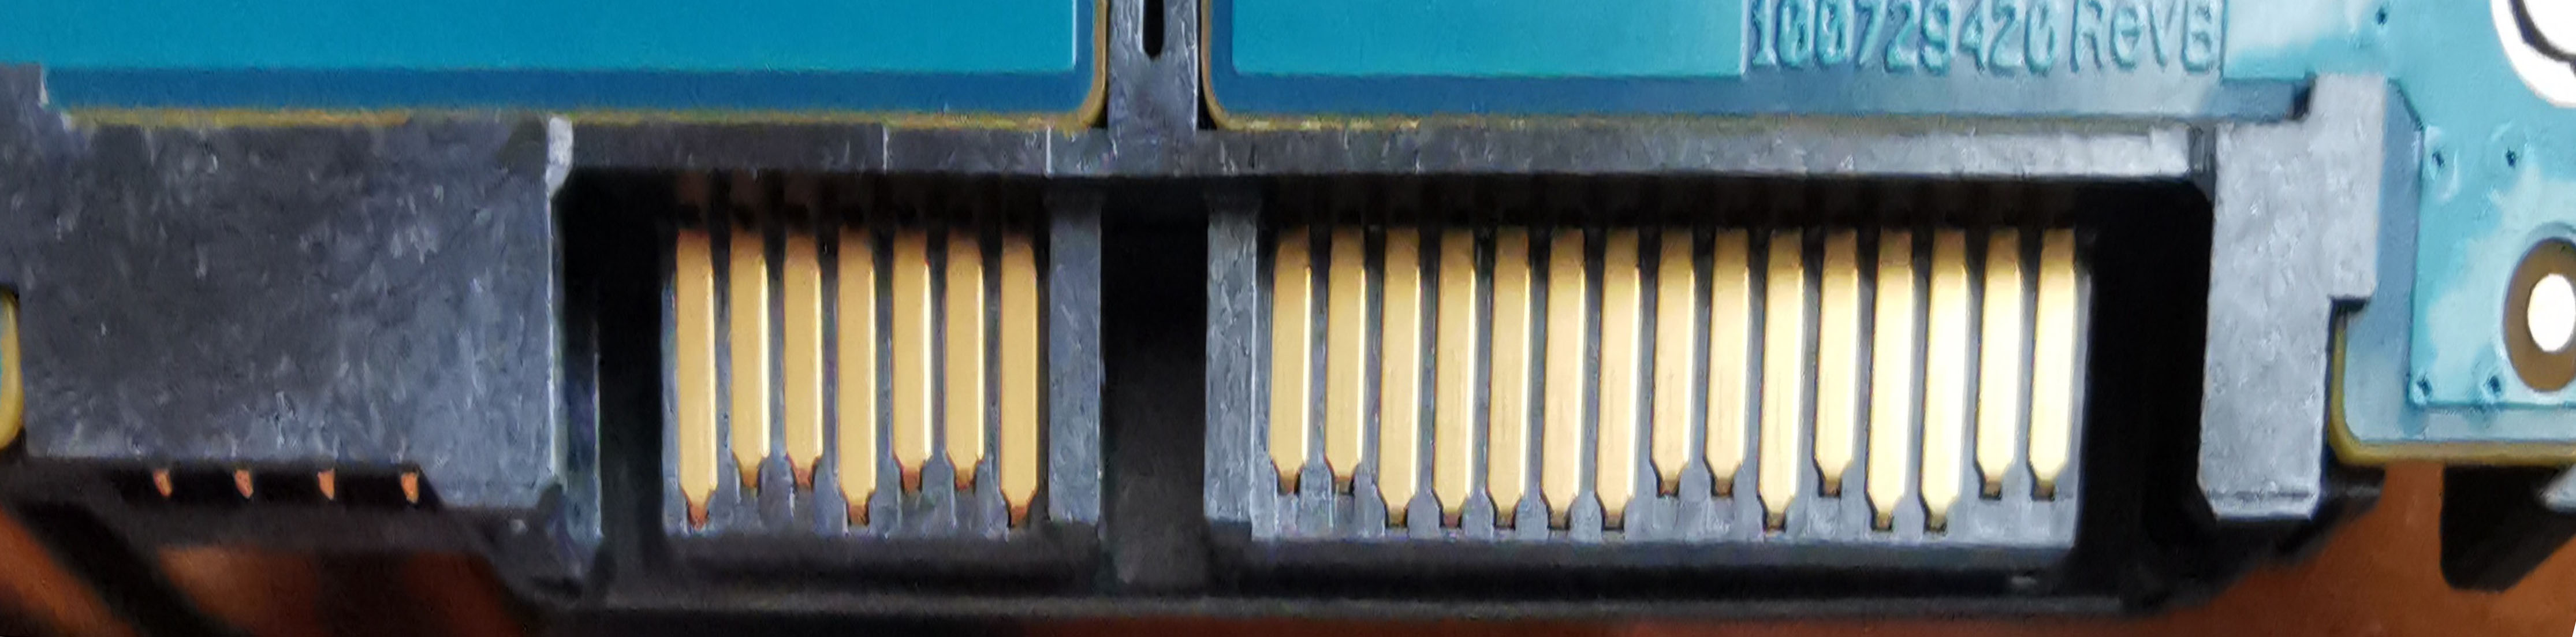
\includegraphics[width=0.7\linewidth]{pic/sata}\\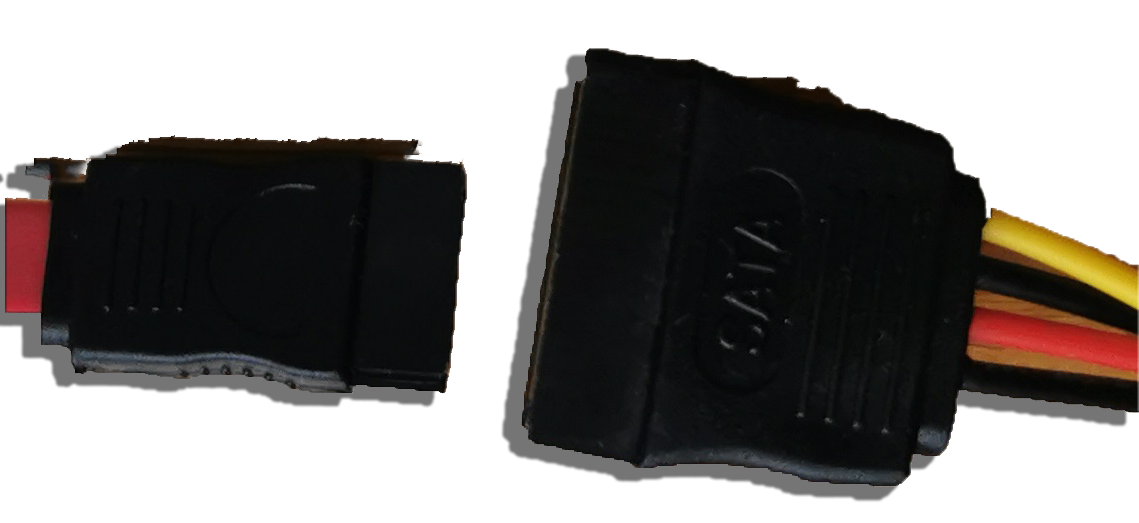
\includegraphics[width=0.7\linewidth]{pic/SATA-Lines}	
	\end{center}
	\item SATA分1.0、2.0、3.0等版本,速率快。它有两排扁形针“金手指”,分别是数据接口(左)和电源接口。下图是SATA接口以及电源、数据线。
	\begin{center}
		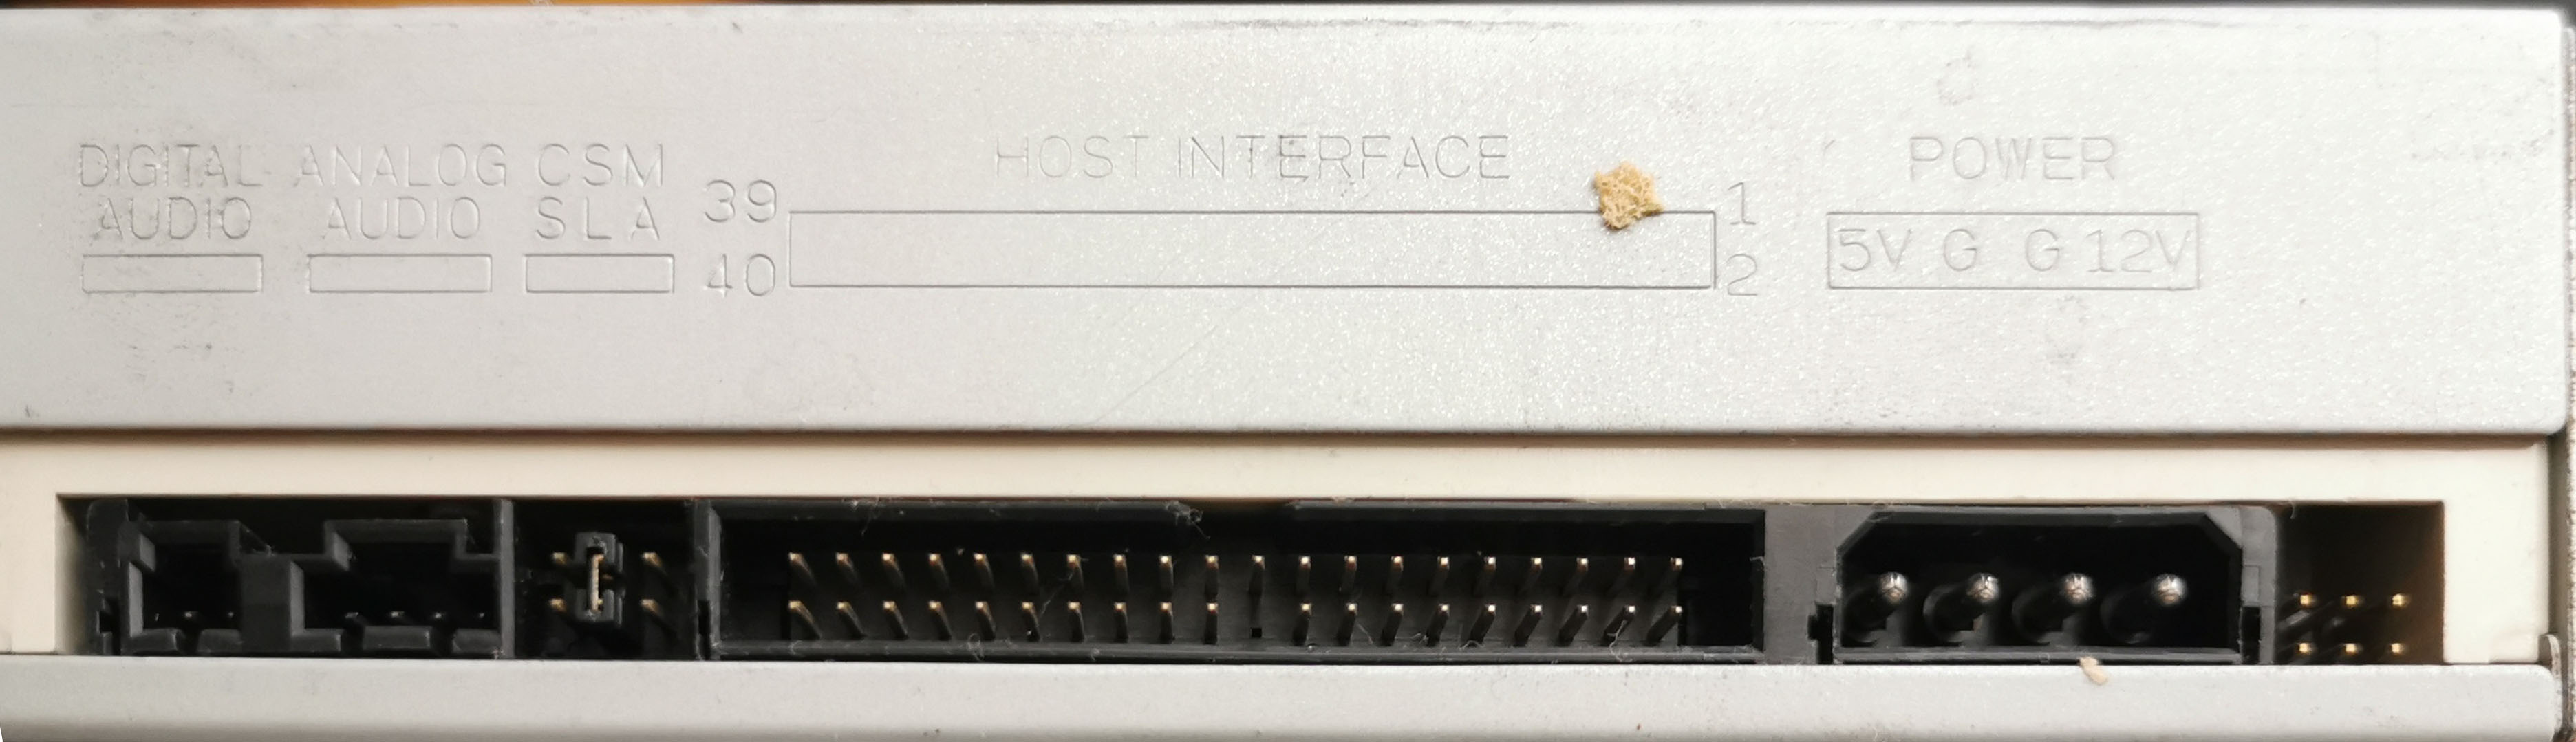
\includegraphics[width=0.7\linewidth]{pic/IDE}
	\end{center}
	\item mSATA(“金手指”分为两段)适用于笔记本。
	\item M.2(“金手指”分为三段)适用于超极本。
\end{enumerate}
再说尺寸。一般我们使用2.5英寸或3.5英寸硬盘。2.5英寸硬盘体积较小,用于笔记本电脑;3.5英存硬盘体积较大,用于台式电脑。一般来说3.5英寸硬盘转速更快,读写速率更大。下图是二者之间的大小对比。
\begin{center}
	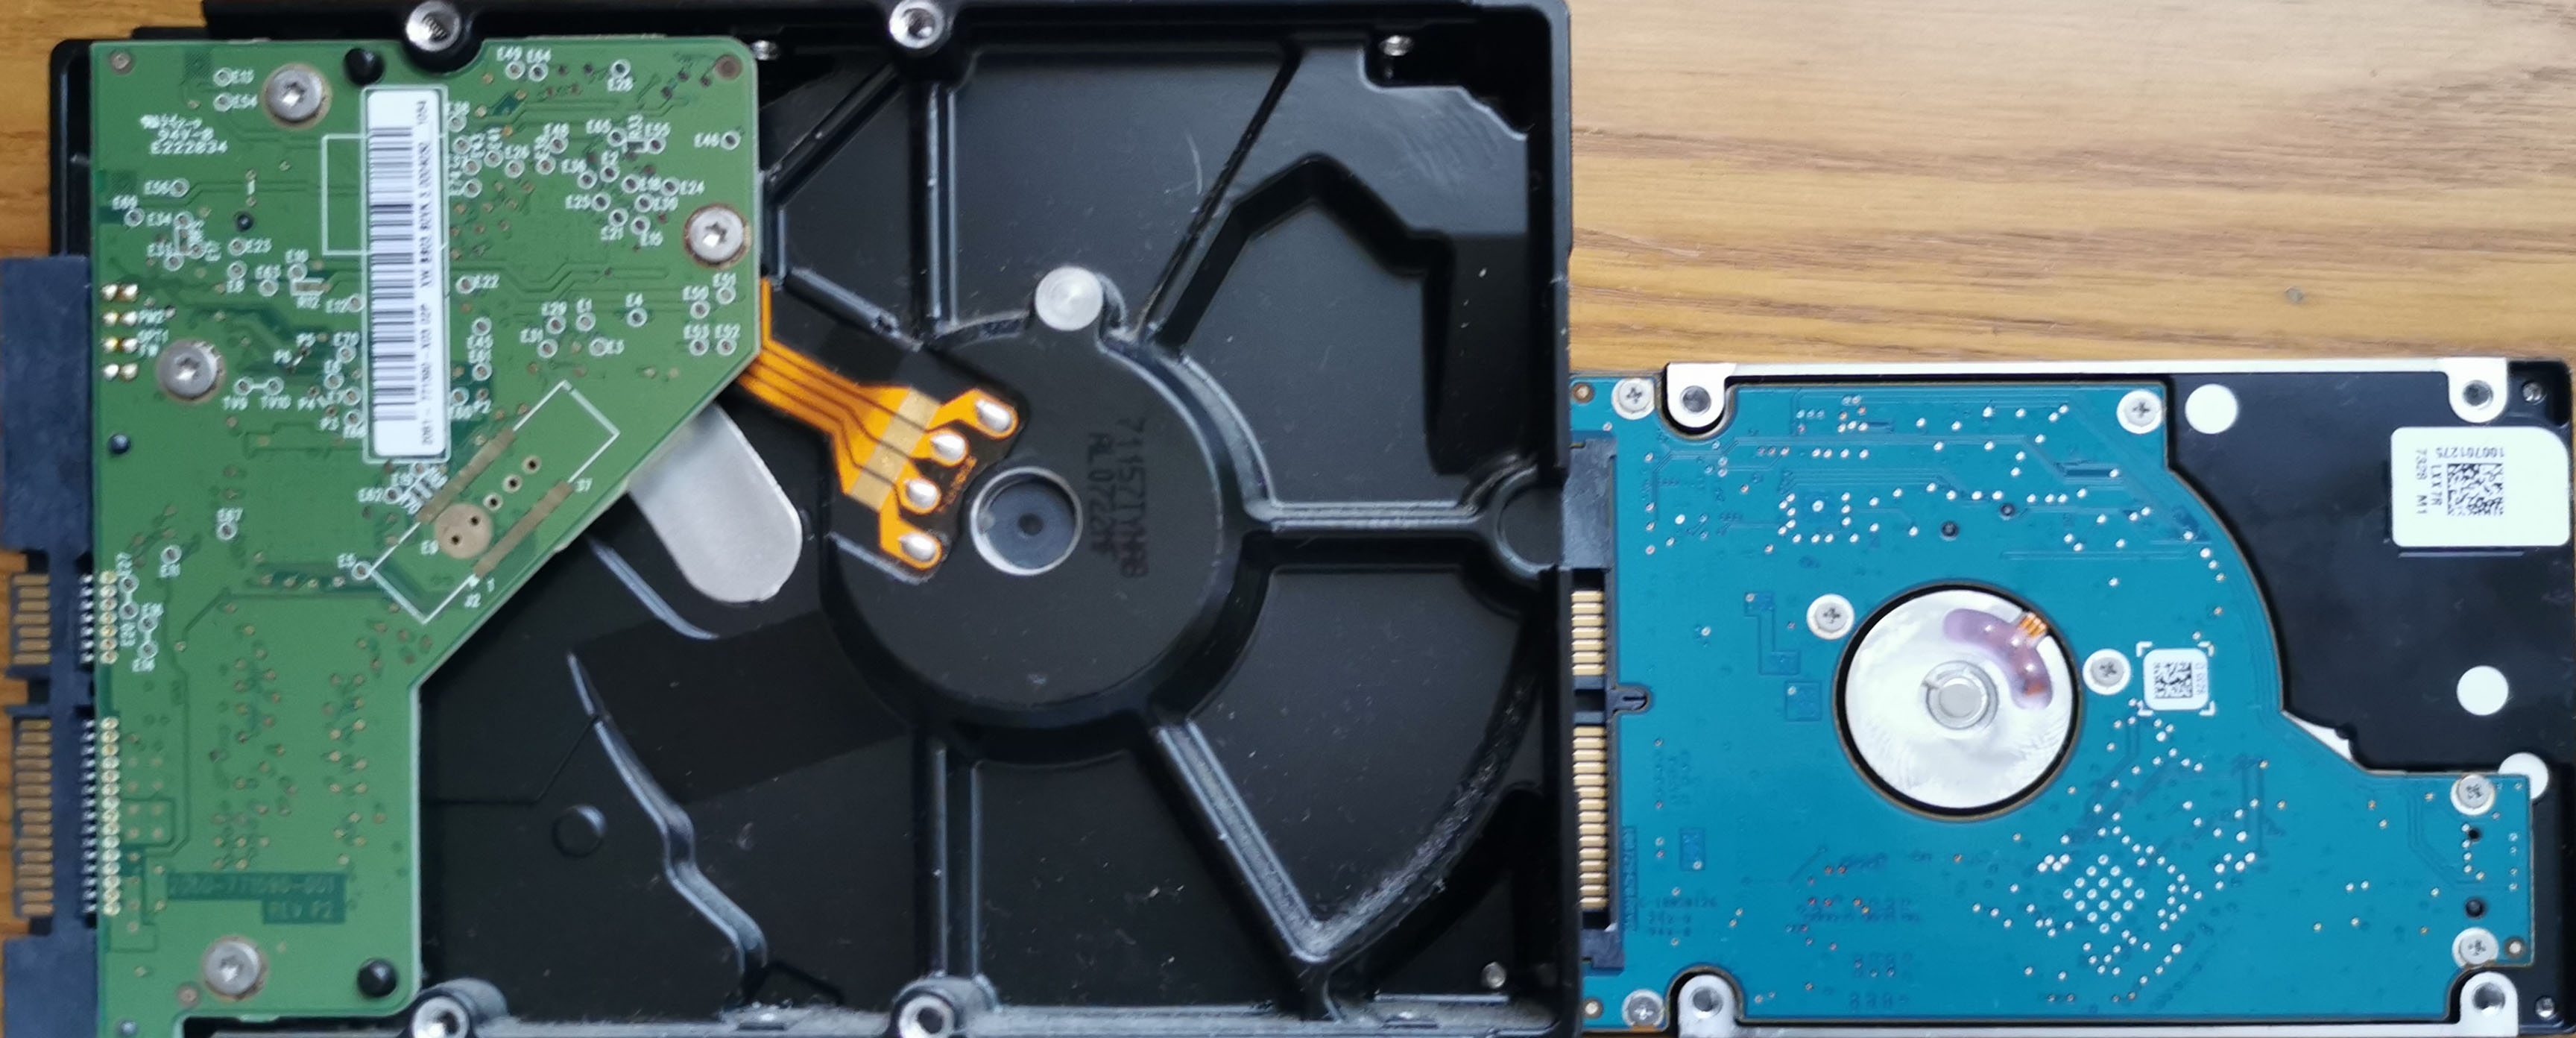
\includegraphics[width=0.7\linewidth]{pic/HD2}\\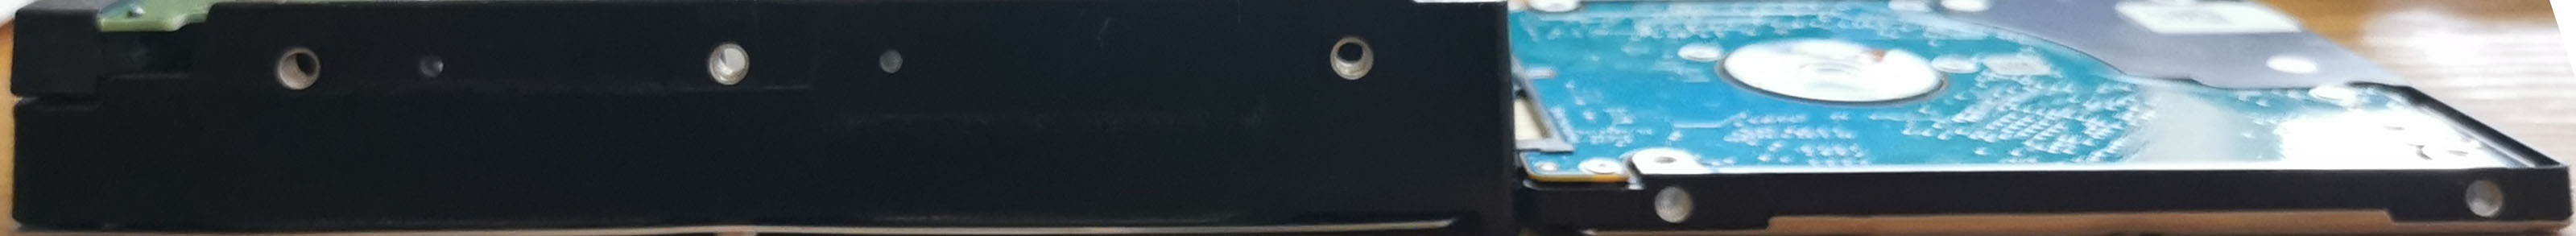
\includegraphics[width=0.7\linewidth]{pic/HD3}	
\end{center} \par
\section{光盘驱动器}
仍然分为内置与外置。外置光驱类似于移动硬盘,而内置光驱类似于内置硬盘。
\chapter{操作系统}
操作系统是一种可用于使用户得以与计算机交流,承载其它计算机程序的计算机程序,因此计算机必须安装操作系统才能运行。无论是国内还是国外,多种优秀的操作系统都可以为我们所用。通常我们使用Windows 操作系统来完成日常事务,GNU/Linux搭建服务器。我们将个人计算机操作系统大致分为两类:桌面操作系统与服务器操作系统。这一节介绍桌面操作系统为主。
\section{-基本概念及操作}
\subsection{屏幕(Screen)}
现在你已经安装好了Windows10操作系统。首先你需要知道什么是“屏幕”。我们将你在显示器上看到的部分称为“屏幕”。就像这样:
\begin{center}
	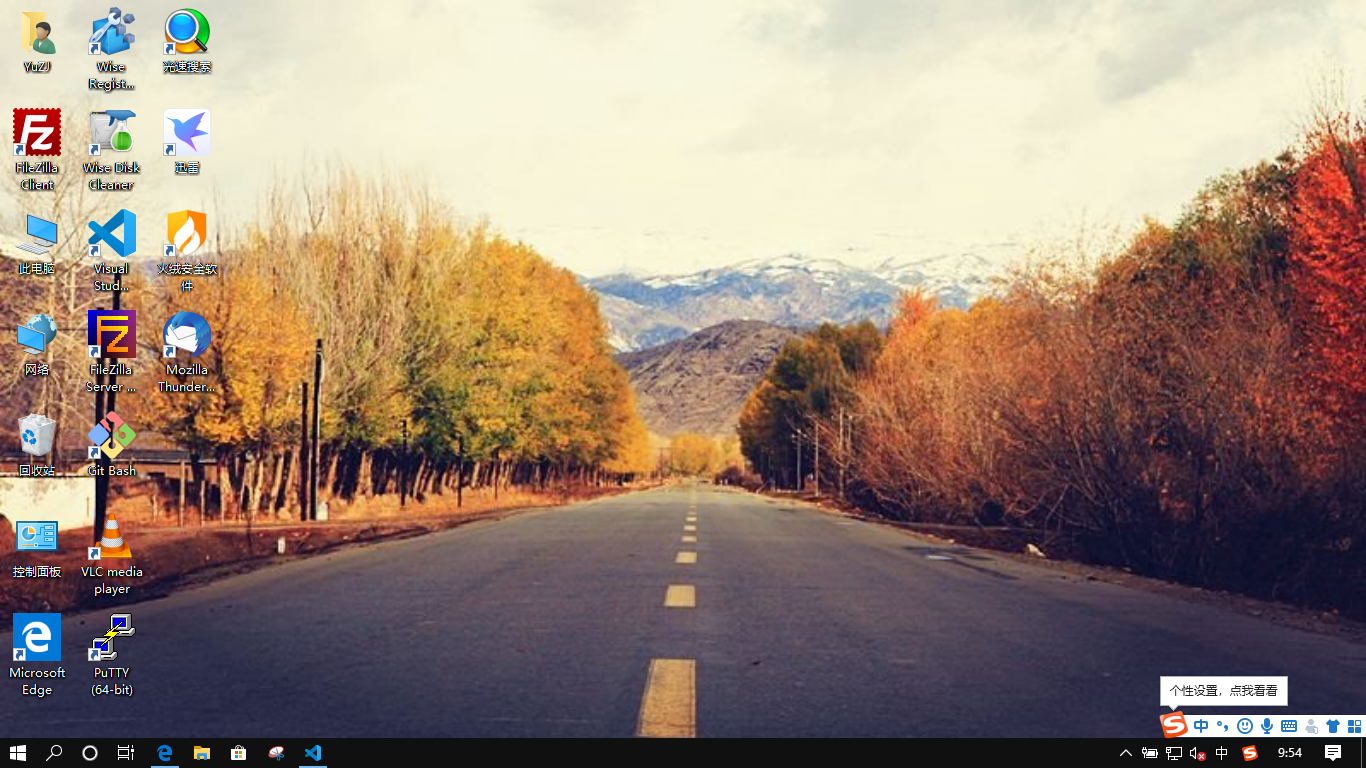
\includegraphics[width=0.7\linewidth]{pic/screen}
\end{center} \par
这就是一个“屏幕”。现在请观察一下线路连接。如果你使用的是教室内的带投影的台式计算机,你会发现由计算机上的VGA口连出了一条较粗的电缆到中央控制器的VGA口。另几条电缆由类似的接口连接到投影仪和显示器。这种情况下你会发现显示器上的图像与投影仪上的图像几乎是同步的。此时我们将其计算做一个屏幕。\par
如果你连接到多台显示器,你会得到几个屏幕?答案不一定相同。你可以进入“设置”-“显示”查看情况。你会发现“多显示器设置”菜单有多种选择——“复制”(就是指将主显示器上的图像复制到副显示器上面,常见的有两个显示器的柜台机就是这种构造)与“扩展”(相当于把副显示器与主显示器合二为一形成了一块较大的屏幕)。效果如下图所示。我们将第一种情况认定为1块屏幕,第二种两块。
\begin{center}
	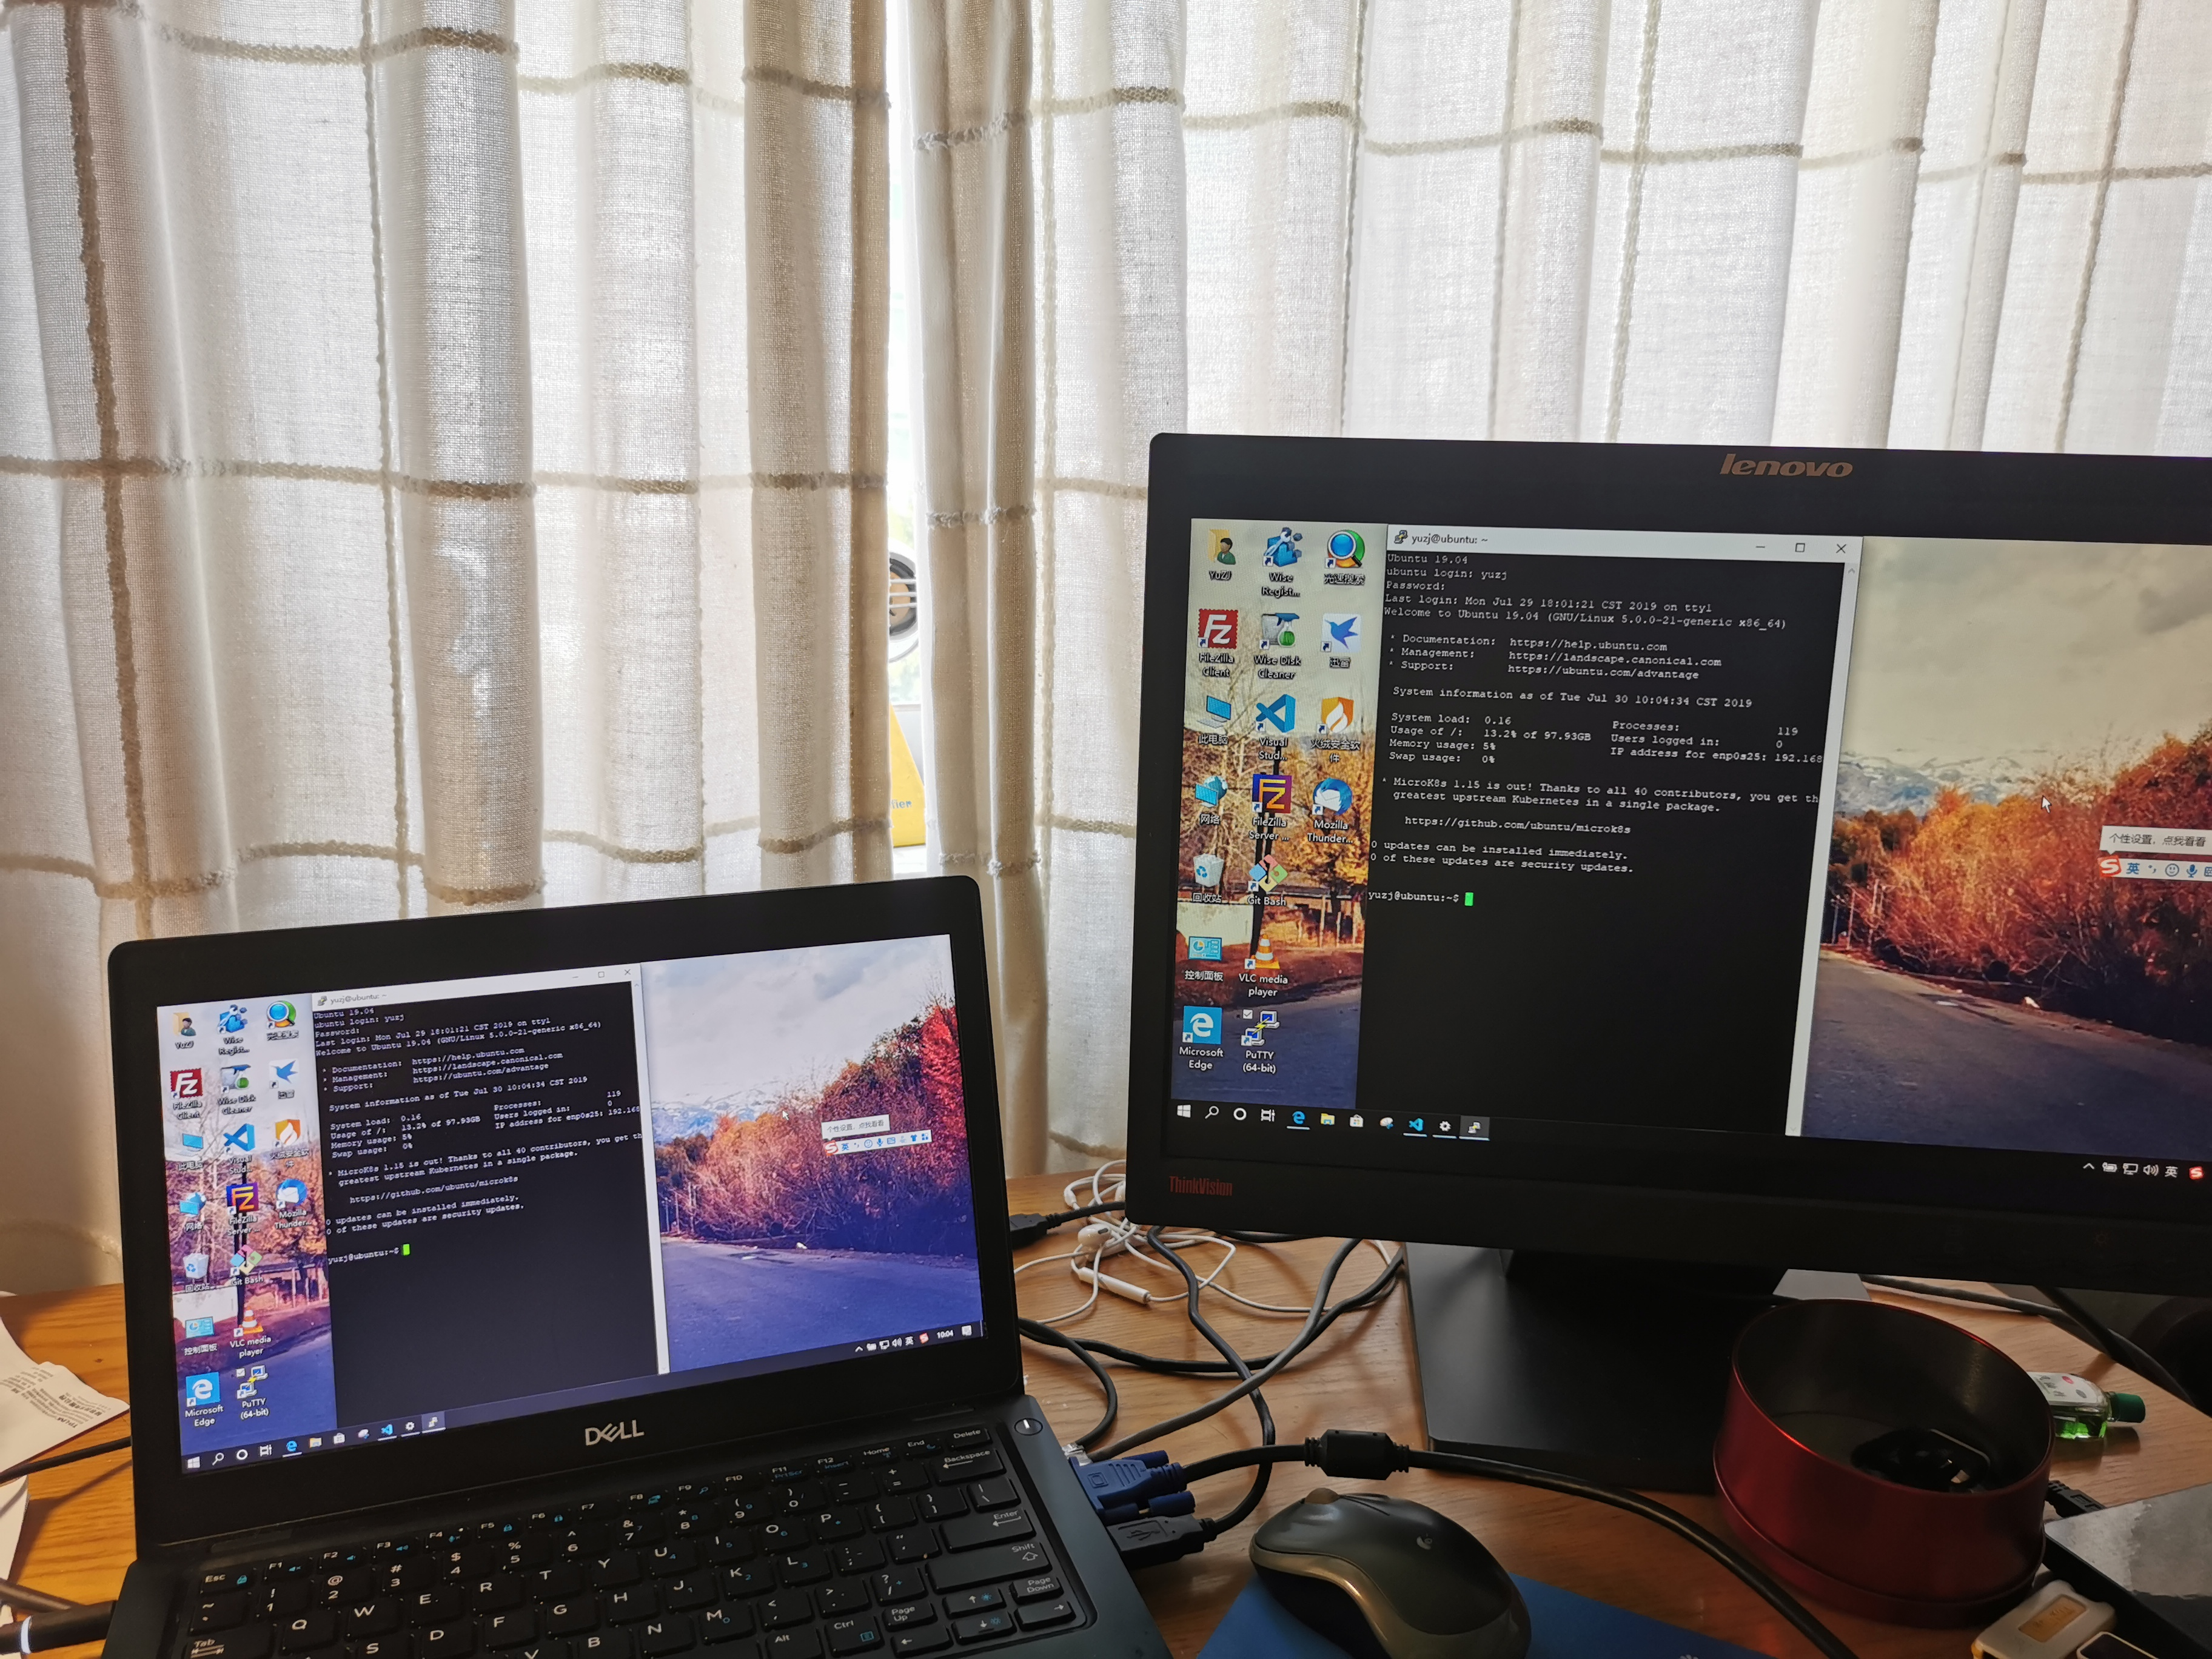
\includegraphics[width=0.7\linewidth]{pic/ScrCopy}\\
	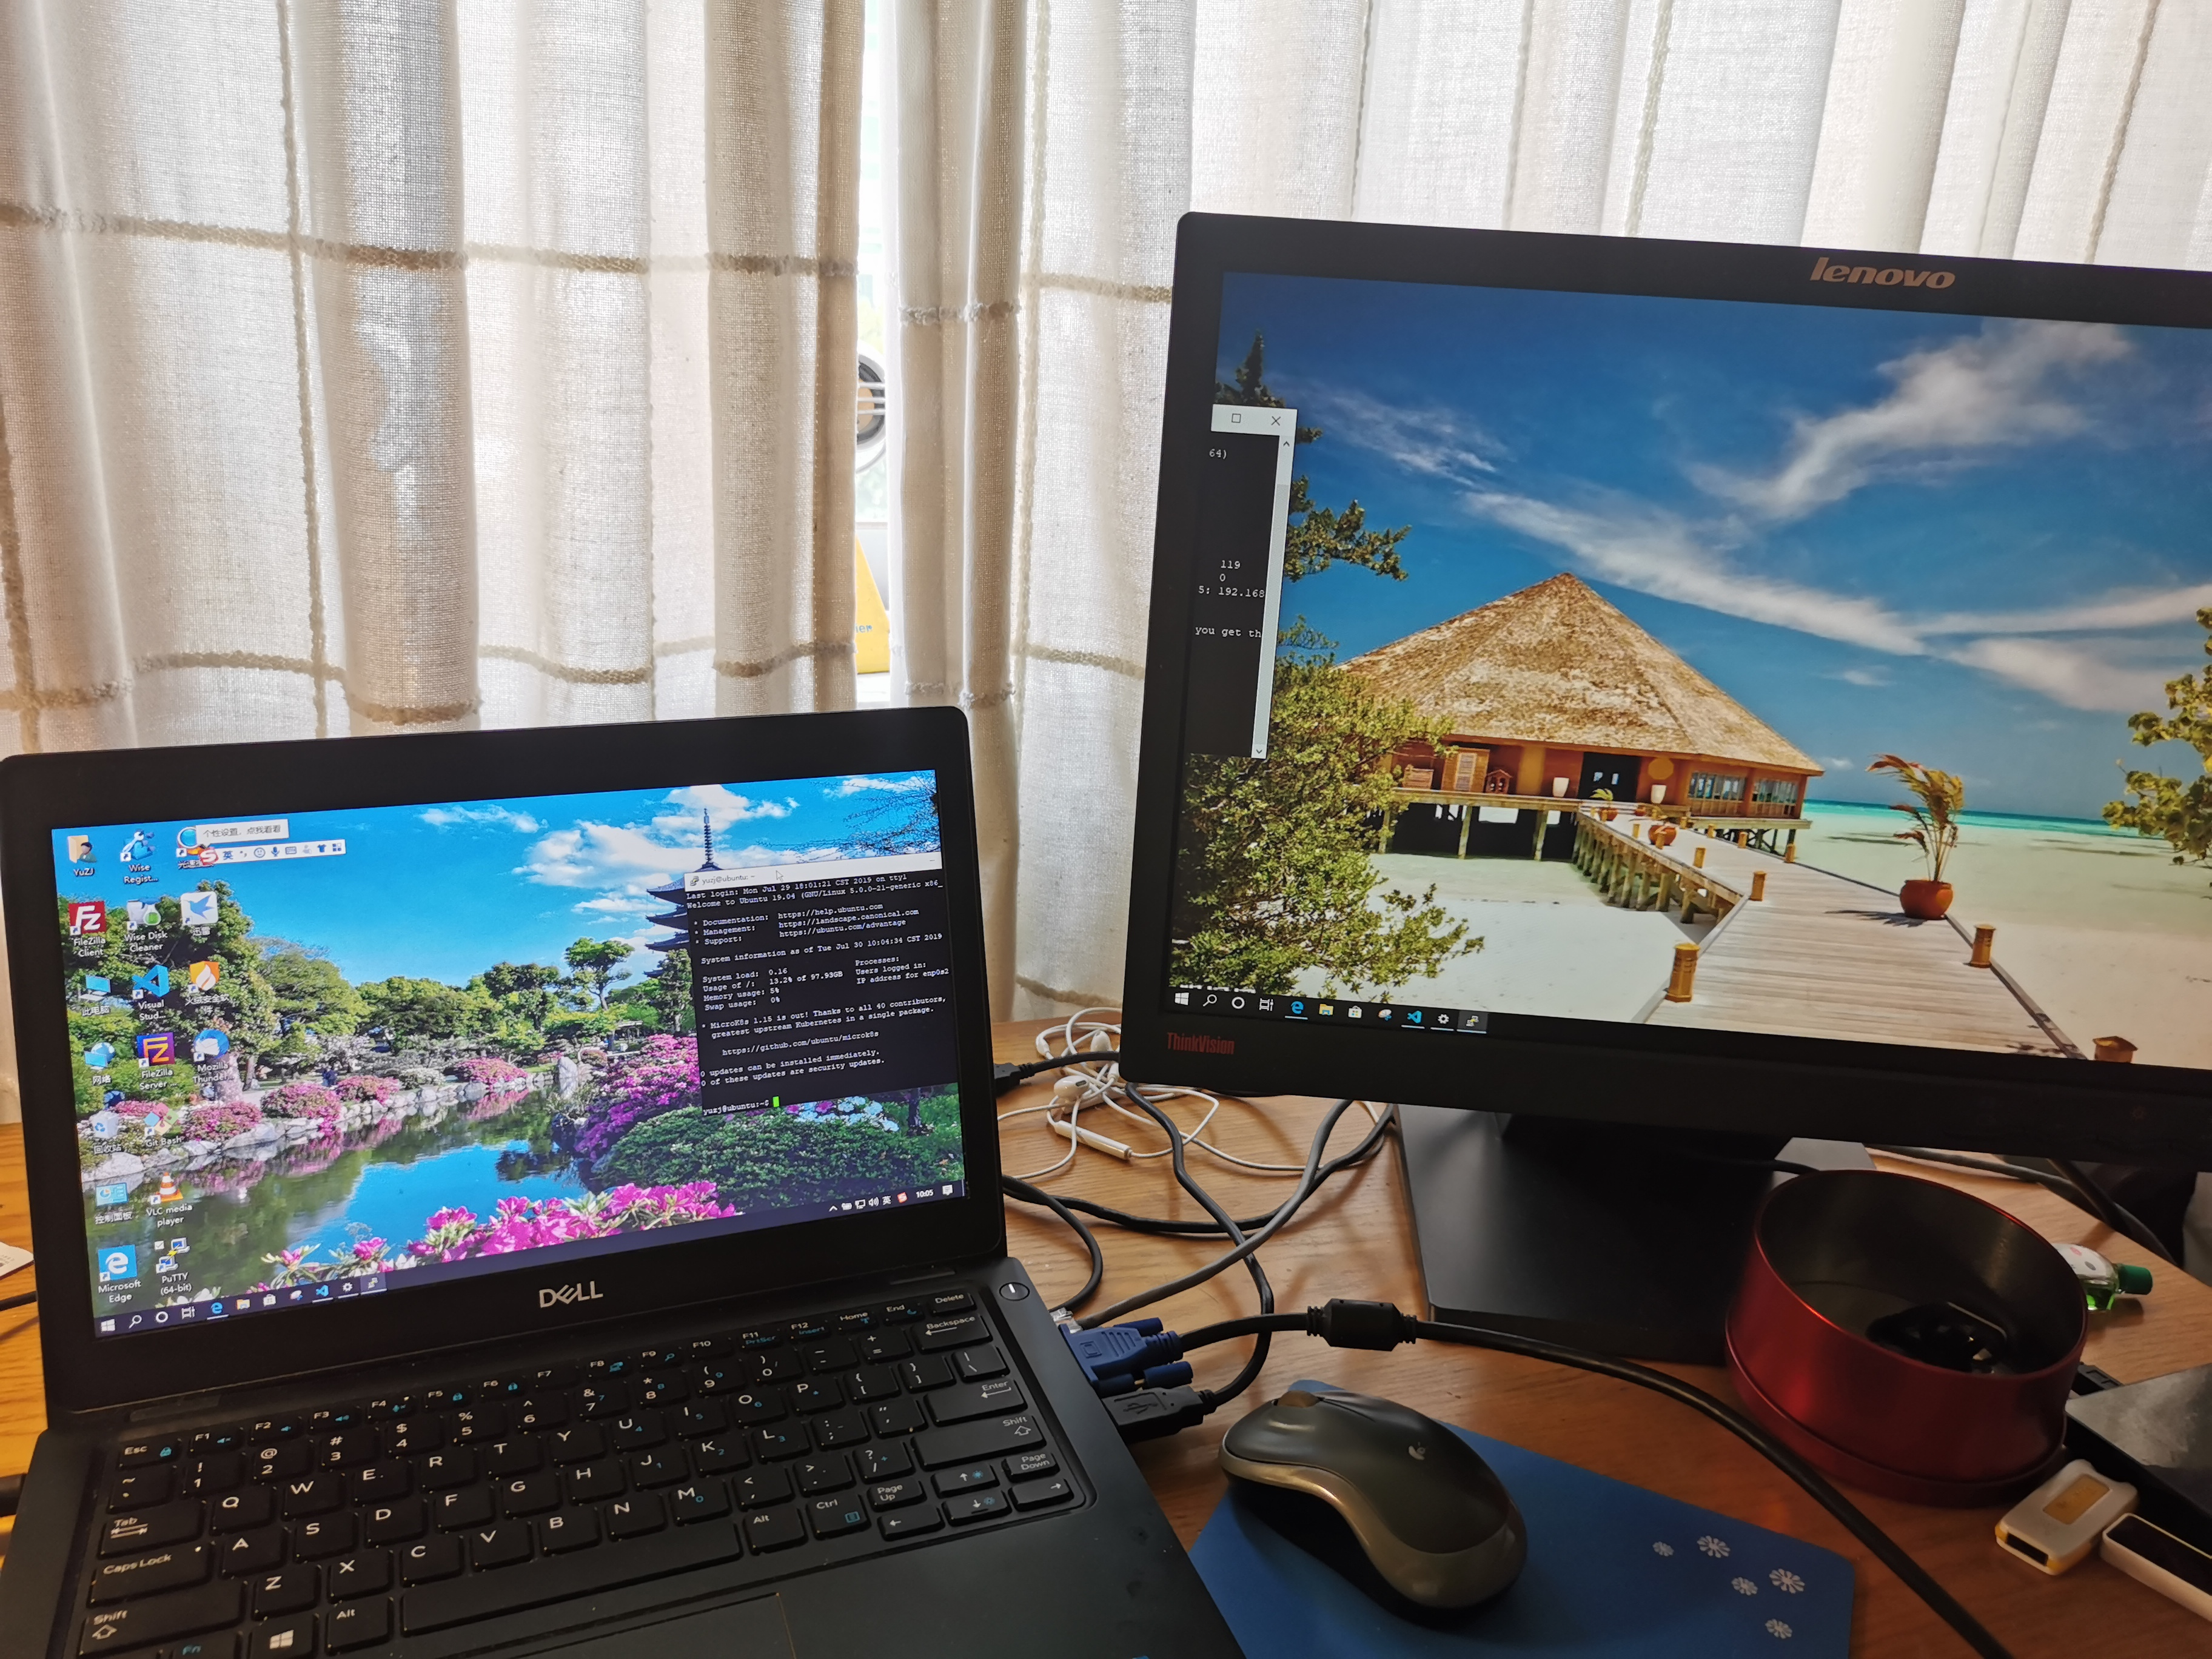
\includegraphics[width=0.7\linewidth]{pic/ScrExtend}
\end{center} 
\subsection{桌面(Desktop)、任务栏与开始菜单}
\begin{center}
	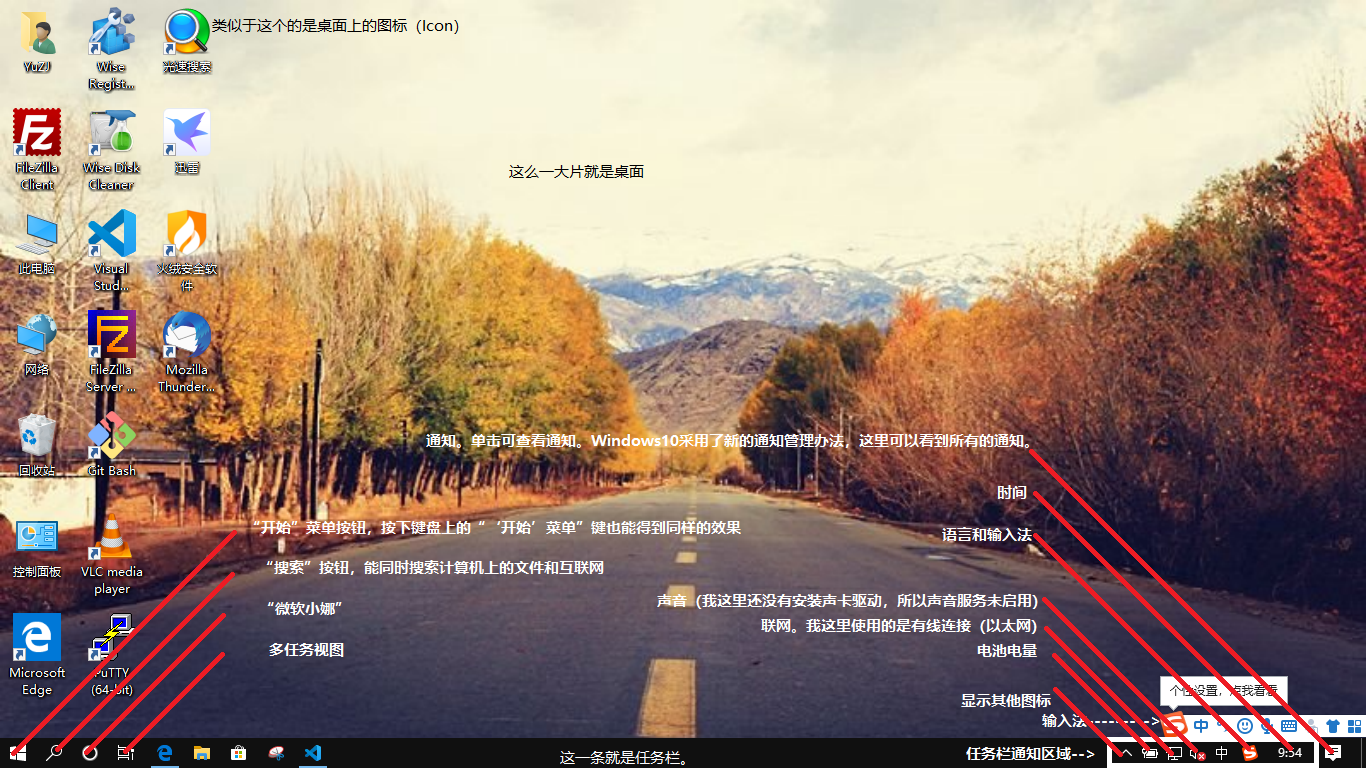
\includegraphics[scale=0.4,angle=90]{pic/screenIntro}
\end{center} \par
上图大致地概括了桌面、任务栏与开始菜单的组成部分。你可以自定义任务栏上显示什么图标。方法:在任务栏上右击-“任务栏设置”-“选择哪些图标显示在任务栏上”。
\subsection{窗口(Window/Form)}
\label{sec:Frm}
我们把屏幕上的一个一个独立的矩形区域称作“窗口”。例如,这就是一个窗口:
\begin{center}
	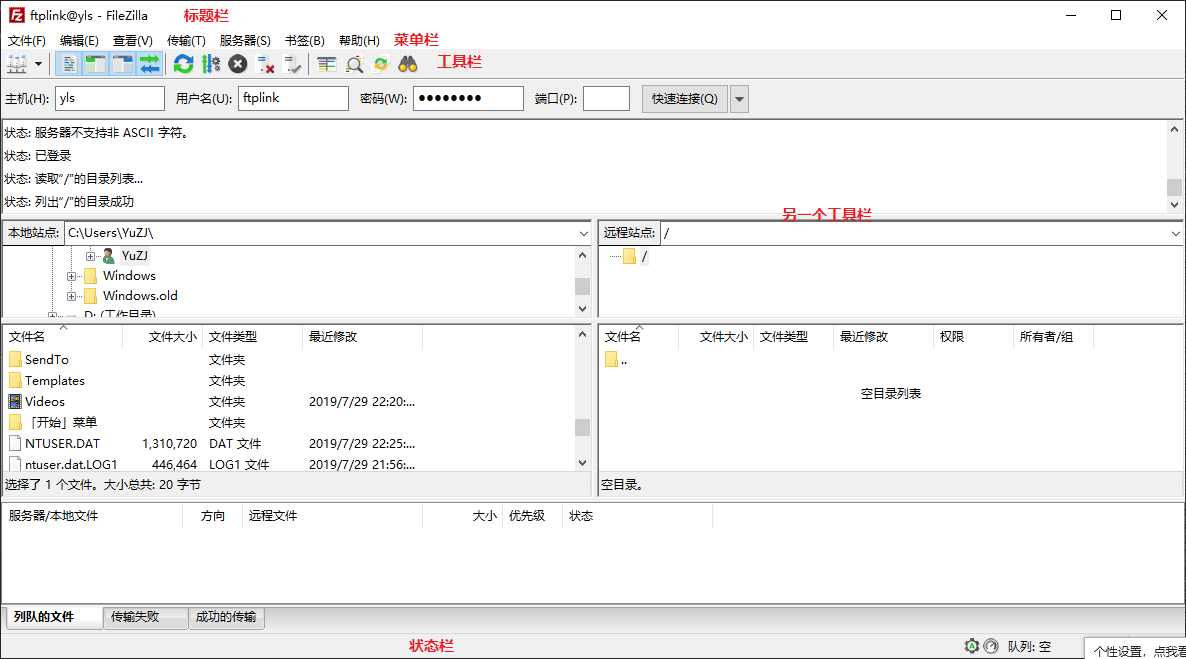
\includegraphics[width=0.7\linewidth]{pic/kj1}
\end{center} \par
一个窗口上面又有许多独立的组成要素,我们把它称为“控件”。常见的控件如下:
\begin{center}
	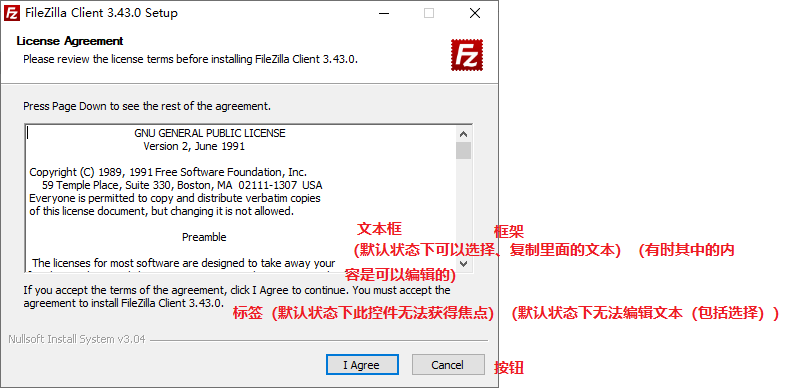
\includegraphics[width=0.7\linewidth]{pic/kj2}\\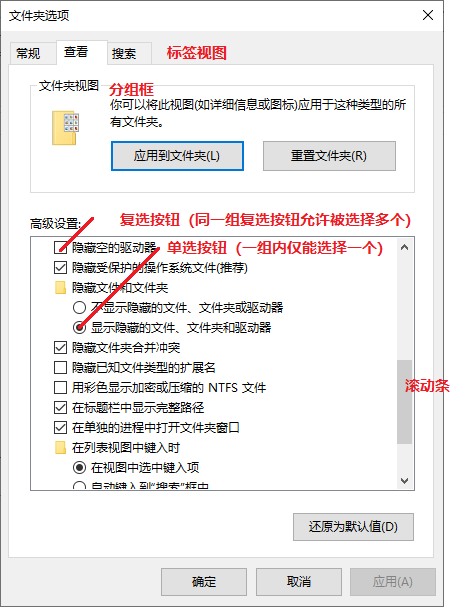
\includegraphics[width=0.7\linewidth]{pic/kj3}
\end{center} \par
现在请回到“键盘”学习如何使用快捷键。注意,有时它们又被称为“窗体”或“窗格”。
\subsection{文件(File)、目录(Directory)、路径(Path)与文件夹(Folder)}
简单地说,你在“文件资源管理器”上看到的不是文件夹的就是文件。文件夹在“详细信息”窗口与“属性”菜单中被清楚地标明“文件夹”。文件夹可以包含文件。现阶段你可以理解“文件夹”就是“目录”,虽然两者实质上是有区别的(目录是列表,文件夹是对象)。“路径”就是文件夹或者文件的“位置”,是一个字符串,如“C:\textbackslash Users\textbackslash SGComputers\textbackslash AppData\textbackslash Roaming\textbackslash Adobe\textbackslash Flash Player\textbackslash NativeCache”。Windows上使用“计算机-磁盘-文件(夹)”来管理文件。它们的路径包含设备卷标,如“D:\textbackslash”。关于绝对路径与相对路径你可以参考\pageref{sec:path}页的\ref{sec:path}。
\subsection{系统的关键位置}
目前阶段,这些关键位置的文件希望你不要操作:
\begin{enumerate}
	\item C:\textbackslash Windows  Windows操作系统放置系统可执行文件的地方。
	\item C:\textbackslash Windows\textbackslash System32  也是Windows操作系统放置系统可执行文件的地方。
\end{enumerate}\par
这些位置也比较重要:
\begin{enumerate}
	\item C:\textbackslash Program Files Windows操作系统应用程序的安装目录。这里安装的程序默认是可以被所有用户使用的。
	\item C:\textbackslash Program Files (x86) 如果你有这个目录,那么你的操作系统就是64位的。这里放置了32位应用程序的安装目录,而上一条中的目录是给64位程序使用的。如果没有,那么你的操作系统就是32位的。上一条中的目录是给32位程序使用的。
	\item C:\textbackslash ProgramData  存放在以上两个目录中的应用程序存放数据文件的地方。这里经常会有卸载残留,需要手动清扫(警告!只是删除自己熟悉且完全确定的目录)。
	\item C:\textbackslash Windows.old  老版本Windows的目录,如果不要回退到以前的版本你可以删除它(不要在“文件资源管理器”中删除——使用“开始”菜单-“Windows管理工具”-“磁盘清理”,使用管理员权限运行清理,删除“以前的Windows安装”)。
\end{enumerate}
\subsection{可执行文件(Executables)}
\label{sec:exe}一般扩展名为*.EXE,*.dll(Windows运行库文件)或*.COM(MS DOS可执行文件)等。一般地,仅二进制文件可在Windows操作系统上运行。虽然*.BAT(批处理文件。你可以把多个命令写入一个批处理文件并让Windows按照预定次序,满足预定条件地一次执行所有命令),*.CMD(类似于批处理文件,支持更多的命令,仅在Windows2000以上可用),*.VBS(VB Script,一种类似于VB的脚本语言),*.VBE(加密的VBS),*.JS(Java Script),*.JSE(不用说了吧),*.WSF,*.WSH,*.MSC(微软控制台文件)等文件也可直接在Windows操作系统上运行,但他们需要解释器。\par
可执行文件是系统必须的(系统启动的关键进程也是靠可执行文件完成的——你的桌面其实也是一个可执行文件的进程),但也是危险的。因此请不要删除系统关键位置的可执行文件(当然我也不相信你删得掉——有个叫做System的用户会阻止你的如果出现了病毒,反病毒软件会帮你删除的)并{\color{red}千万别双击自己不明白的可执行文件!!!!!!}下一节将会教你修改“文件资源管理器”的相关设置以防范虚假扩展名欺骗。
\subsection{-快捷方式}
快捷方式指的是一个指向目标文件的链接。

